\documentclass[twoside]{book}

% Packages required by doxygen
\usepackage{fixltx2e}
\usepackage{calc}
\usepackage{doxygen}
\usepackage[export]{adjustbox} % also loads graphicx
\usepackage{graphicx}
\usepackage[utf8]{inputenc}
\usepackage{makeidx}
\usepackage{multicol}
\usepackage{multirow}
\PassOptionsToPackage{warn}{textcomp}
\usepackage{textcomp}
\usepackage[nointegrals]{wasysym}
\usepackage[table]{xcolor}

% Font selection
\usepackage[T1]{fontenc}
\usepackage[scaled=.90]{helvet}
\usepackage{courier}
\usepackage{amssymb}
\usepackage{sectsty}
\renewcommand{\familydefault}{\sfdefault}
\allsectionsfont{%
  \fontseries{bc}\selectfont%
  \color{darkgray}%
}
\renewcommand{\DoxyLabelFont}{%
  \fontseries{bc}\selectfont%
  \color{darkgray}%
}
\newcommand{\+}{\discretionary{\mbox{\scriptsize$\hookleftarrow$}}{}{}}

% Page & text layout
\usepackage{geometry}
\geometry{%
  a4paper,%
  top=2.5cm,%
  bottom=2.5cm,%
  left=2.5cm,%
  right=2.5cm%
}
\tolerance=750
\hfuzz=15pt
\hbadness=750
\setlength{\emergencystretch}{15pt}
\setlength{\parindent}{0cm}
\setlength{\parskip}{3ex plus 2ex minus 2ex}
\makeatletter
\renewcommand{\paragraph}{%
  \@startsection{paragraph}{4}{0ex}{-1.0ex}{1.0ex}{%
    \normalfont\normalsize\bfseries\SS@parafont%
  }%
}
\renewcommand{\subparagraph}{%
  \@startsection{subparagraph}{5}{0ex}{-1.0ex}{1.0ex}{%
    \normalfont\normalsize\bfseries\SS@subparafont%
  }%
}
\makeatother

% Headers & footers
\usepackage{fancyhdr}
\pagestyle{fancyplain}
\fancyhead[LE]{\fancyplain{}{\bfseries\thepage}}
\fancyhead[CE]{\fancyplain{}{}}
\fancyhead[RE]{\fancyplain{}{\bfseries\leftmark}}
\fancyhead[LO]{\fancyplain{}{\bfseries\rightmark}}
\fancyhead[CO]{\fancyplain{}{}}
\fancyhead[RO]{\fancyplain{}{\bfseries\thepage}}
\fancyfoot[LE]{\fancyplain{}{}}
\fancyfoot[CE]{\fancyplain{}{}}
\fancyfoot[RE]{\fancyplain{}{\bfseries\scriptsize Generated by Doxygen }}
\fancyfoot[LO]{\fancyplain{}{\bfseries\scriptsize Generated by Doxygen }}
\fancyfoot[CO]{\fancyplain{}{}}
\fancyfoot[RO]{\fancyplain{}{}}
\renewcommand{\footrulewidth}{0.4pt}
\renewcommand{\chaptermark}[1]{%
  \markboth{#1}{}%
}
\renewcommand{\sectionmark}[1]{%
  \markright{\thesection\ #1}%
}

% Indices & bibliography
\usepackage{natbib}
\usepackage[titles]{tocloft}
\setcounter{tocdepth}{3}
\setcounter{secnumdepth}{5}
\makeindex

% Hyperlinks (required, but should be loaded last)
\usepackage{ifpdf}
\ifpdf
  \usepackage[pdftex,pagebackref=true]{hyperref}
\else
  \usepackage[ps2pdf,pagebackref=true]{hyperref}
\fi
\hypersetup{%
  colorlinks=true,%
  linkcolor=blue,%
  citecolor=blue,%
  unicode%
}

% Custom commands
\newcommand{\clearemptydoublepage}{%
  \newpage{\pagestyle{empty}\cleardoublepage}%
}

\usepackage{caption}
\captionsetup{labelsep=space,justification=centering,font={bf},singlelinecheck=off,skip=4pt,position=top}

%===== C O N T E N T S =====

\begin{document}

% Titlepage & ToC
\hypersetup{pageanchor=false,
             bookmarksnumbered=true,
             pdfencoding=unicode
            }
\pagenumbering{alph}
\begin{titlepage}
\vspace*{7cm}
\begin{center}%
{\Large Space Invaders }\\
\vspace*{1cm}
{\large Generated by Doxygen 1.8.13}\\
\end{center}
\end{titlepage}
\clearemptydoublepage
\pagenumbering{roman}
\tableofcontents
\clearemptydoublepage
\pagenumbering{arabic}
\hypersetup{pageanchor=true}

%--- Begin generated contents ---
\chapter{Hierarchical Index}
\section{Class Hierarchy}
This inheritance list is sorted roughly, but not completely, alphabetically\+:\begin{DoxyCompactList}
\item \contentsline{section}{util\+:\+:Clock}{\pageref{classutil_1_1Clock}}{}
\item \contentsline{section}{util\+:\+:Collision}{\pageref{classutil_1_1Collision}}{}
\item \contentsline{section}{entities\+:\+:Controller}{\pageref{classentities_1_1Controller}}{}
\begin{DoxyCompactList}
\item \contentsline{section}{entities\+:\+:enemies\+:\+:green\+\_\+alien\+:\+:Green\+Alien\+Controller}{\pageref{classentities_1_1enemies_1_1green__alien_1_1GreenAlienController}}{}
\item \contentsline{section}{entities\+:\+:enemies\+:\+:purple\+\_\+alien\+:\+:Purple\+Alien\+Controller}{\pageref{classentities_1_1enemies_1_1purple__alien_1_1PurpleAlienController}}{}
\item \contentsline{section}{entities\+:\+:enemies\+:\+:red\+\_\+alien\+:\+:Red\+Alien\+Controller}{\pageref{classentities_1_1enemies_1_1red__alien_1_1RedAlienController}}{}
\item \contentsline{section}{entities\+:\+:playership\+:\+:Player\+Ship\+Controller}{\pageref{classentities_1_1playership_1_1PlayerShipController}}{}
\item \contentsline{section}{entities\+:\+:projectiles\+:\+:standard\+:\+:Standard\+Projectile\+Controller}{\pageref{classentities_1_1projectiles_1_1standard_1_1StandardProjectileController}}{}
\item \contentsline{section}{entities\+:\+:projectiles\+:\+:standard\+\_\+enemy\+:\+:Standard\+Enemy\+Projectile\+Controller}{\pageref{classentities_1_1projectiles_1_1standard__enemy_1_1StandardEnemyProjectileController}}{}
\item \contentsline{section}{entities\+:\+:shield\+:\+:Shield\+Controller}{\pageref{classentities_1_1shield_1_1ShieldController}}{}
\end{DoxyCompactList}
\item enable\+\_\+shared\+\_\+from\+\_\+this\begin{DoxyCompactList}
\item \contentsline{section}{entities\+:\+:Observer}{\pageref{classentities_1_1Observer}}{}
\begin{DoxyCompactList}
\item \contentsline{section}{entities\+:\+:View}{\pageref{classentities_1_1View}}{}
\begin{DoxyCompactList}
\item \contentsline{section}{entities\+:\+:enemies\+:\+:green\+\_\+alien\+:\+:Green\+Alien\+View}{\pageref{classentities_1_1enemies_1_1green__alien_1_1GreenAlienView}}{}
\item \contentsline{section}{entities\+:\+:enemies\+:\+:purple\+\_\+alien\+:\+:Purple\+Alien\+View}{\pageref{classentities_1_1enemies_1_1purple__alien_1_1PurpleAlienView}}{}
\item \contentsline{section}{entities\+:\+:enemies\+:\+:red\+\_\+alien\+:\+:Red\+Alien\+View}{\pageref{classentities_1_1enemies_1_1red__alien_1_1RedAlienView}}{}
\item \contentsline{section}{entities\+:\+:playership\+:\+:Player\+Lives\+View}{\pageref{classentities_1_1playership_1_1PlayerLivesView}}{}
\item \contentsline{section}{entities\+:\+:playership\+:\+:Player\+Ship\+View}{\pageref{classentities_1_1playership_1_1PlayerShipView}}{}
\item \contentsline{section}{entities\+:\+:projectiles\+:\+:standard\+:\+:Standard\+Projectile\+View}{\pageref{classentities_1_1projectiles_1_1standard_1_1StandardProjectileView}}{}
\item \contentsline{section}{entities\+:\+:projectiles\+:\+:standard\+\_\+enemy\+:\+:Standard\+Enemy\+Projectile\+View}{\pageref{classentities_1_1projectiles_1_1standard__enemy_1_1StandardEnemyProjectileView}}{}
\item \contentsline{section}{entities\+:\+:shield\+:\+:Shield\+View}{\pageref{classentities_1_1shield_1_1ShieldView}}{}
\end{DoxyCompactList}
\item \contentsline{section}{World}{\pageref{classWorld}}{}
\end{DoxyCompactList}
\end{DoxyCompactList}
\item \contentsline{section}{Game}{\pageref{classGame}}{}
\item \contentsline{section}{entities\+:\+:projectiles\+:\+:Projectile\+Factory}{\pageref{classentities_1_1projectiles_1_1ProjectileFactory}}{}
\item \contentsline{section}{Space\+Settings}{\pageref{structSpaceSettings}}{}
\item \contentsline{section}{util\+:\+:Stopwatch}{\pageref{classutil_1_1Stopwatch}}{}
\item \contentsline{section}{entities\+:\+:Subject}{\pageref{classentities_1_1Subject}}{}
\begin{DoxyCompactList}
\item \contentsline{section}{entities\+:\+:Entity}{\pageref{classentities_1_1Entity}}{}
\begin{DoxyCompactList}
\item \contentsline{section}{entities\+:\+:enemies\+:\+:Enemy}{\pageref{classentities_1_1enemies_1_1Enemy}}{}
\begin{DoxyCompactList}
\item \contentsline{section}{entities\+:\+:enemies\+:\+:green\+\_\+alien\+:\+:Green\+Alien}{\pageref{classentities_1_1enemies_1_1green__alien_1_1GreenAlien}}{}
\item \contentsline{section}{entities\+:\+:enemies\+:\+:purple\+\_\+alien\+:\+:Purple\+Alien}{\pageref{classentities_1_1enemies_1_1purple__alien_1_1PurpleAlien}}{}
\item \contentsline{section}{entities\+:\+:enemies\+:\+:red\+\_\+alien\+:\+:Red\+Alien}{\pageref{classentities_1_1enemies_1_1red__alien_1_1RedAlien}}{}
\end{DoxyCompactList}
\item \contentsline{section}{entities\+:\+:playership\+:\+:Player\+Ship}{\pageref{classentities_1_1playership_1_1PlayerShip}}{}
\item \contentsline{section}{entities\+:\+:projectiles\+:\+:standard\+:\+:Standard\+Projectile}{\pageref{classentities_1_1projectiles_1_1standard_1_1StandardProjectile}}{}
\item \contentsline{section}{entities\+:\+:projectiles\+:\+:standard\+\_\+enemy\+:\+:Standard\+Enemy\+Projectile}{\pageref{classentities_1_1projectiles_1_1standard__enemy_1_1StandardEnemyProjectile}}{}
\item \contentsline{section}{entities\+:\+:shield\+:\+:Shield}{\pageref{classentities_1_1shield_1_1Shield}}{}
\end{DoxyCompactList}
\item \contentsline{section}{World}{\pageref{classWorld}}{}
\end{DoxyCompactList}
\item \contentsline{section}{util\+:\+:Transformation}{\pageref{classutil_1_1Transformation}}{}
\end{DoxyCompactList}

\chapter{Class Index}
\section{Class List}
Here are the classes, structs, unions and interfaces with brief descriptions\+:\begin{DoxyCompactList}
\item\contentsline{section}{\hyperlink{classutil_1_1Clock}{util\+::\+Clock} }{\pageref{classutil_1_1Clock}}{}
\item\contentsline{section}{\hyperlink{classutil_1_1Collision}{util\+::\+Collision} }{\pageref{classutil_1_1Collision}}{}
\item\contentsline{section}{\hyperlink{classobjects_1_1Controller}{objects\+::\+Controller} }{\pageref{classobjects_1_1Controller}}{}
\item\contentsline{section}{\hyperlink{classobjects_1_1enemies_1_1Enemy}{objects\+::enemies\+::\+Enemy} }{\pageref{classobjects_1_1enemies_1_1Enemy}}{}
\item\contentsline{section}{\hyperlink{classobjects_1_1enemies_1_1EnemyFactory}{objects\+::enemies\+::\+Enemy\+Factory} }{\pageref{classobjects_1_1enemies_1_1EnemyFactory}}{}
\item\contentsline{section}{\hyperlink{classobjects_1_1Entity}{objects\+::\+Entity} }{\pageref{classobjects_1_1Entity}}{}
\item\contentsline{section}{\hyperlink{classGame}{Game} }{\pageref{classGame}}{}
\item\contentsline{section}{\hyperlink{classobjects_1_1enemies_1_1green__alien_1_1GreenAlien}{objects\+::enemies\+::green\+\_\+alien\+::\+Green\+Alien} }{\pageref{classobjects_1_1enemies_1_1green__alien_1_1GreenAlien}}{}
\item\contentsline{section}{\hyperlink{classobjects_1_1enemies_1_1green__alien_1_1GreenAlienController}{objects\+::enemies\+::green\+\_\+alien\+::\+Green\+Alien\+Controller} }{\pageref{classobjects_1_1enemies_1_1green__alien_1_1GreenAlienController}}{}
\item\contentsline{section}{\hyperlink{classobjects_1_1enemies_1_1green__alien_1_1GreenAlienView}{objects\+::enemies\+::green\+\_\+alien\+::\+Green\+Alien\+View} }{\pageref{classobjects_1_1enemies_1_1green__alien_1_1GreenAlienView}}{}
\item\contentsline{section}{\hyperlink{classobjects_1_1Observer}{objects\+::\+Observer} }{\pageref{classobjects_1_1Observer}}{}
\item\contentsline{section}{\hyperlink{classobjects_1_1playership_1_1PlayerLivesView}{objects\+::playership\+::\+Player\+Lives\+View} }{\pageref{classobjects_1_1playership_1_1PlayerLivesView}}{}
\item\contentsline{section}{\hyperlink{classobjects_1_1playership_1_1PlayerShip}{objects\+::playership\+::\+Player\+Ship} }{\pageref{classobjects_1_1playership_1_1PlayerShip}}{}
\item\contentsline{section}{\hyperlink{classobjects_1_1playership_1_1PlayerShipController}{objects\+::playership\+::\+Player\+Ship\+Controller} }{\pageref{classobjects_1_1playership_1_1PlayerShipController}}{}
\item\contentsline{section}{\hyperlink{classobjects_1_1playership_1_1PlayerShipView}{objects\+::playership\+::\+Player\+Ship\+View} }{\pageref{classobjects_1_1playership_1_1PlayerShipView}}{}
\item\contentsline{section}{\hyperlink{classobjects_1_1projectiles_1_1ProjectileFactory}{objects\+::projectiles\+::\+Projectile\+Factory} }{\pageref{classobjects_1_1projectiles_1_1ProjectileFactory}}{}
\item\contentsline{section}{\hyperlink{classobjects_1_1enemies_1_1purple__alien_1_1PurpleAlien}{objects\+::enemies\+::purple\+\_\+alien\+::\+Purple\+Alien} }{\pageref{classobjects_1_1enemies_1_1purple__alien_1_1PurpleAlien}}{}
\item\contentsline{section}{\hyperlink{classobjects_1_1enemies_1_1purple__alien_1_1PurpleAlienController}{objects\+::enemies\+::purple\+\_\+alien\+::\+Purple\+Alien\+Controller} }{\pageref{classobjects_1_1enemies_1_1purple__alien_1_1PurpleAlienController}}{}
\item\contentsline{section}{\hyperlink{classobjects_1_1enemies_1_1purple__alien_1_1PurpleAlienView}{objects\+::enemies\+::purple\+\_\+alien\+::\+Purple\+Alien\+View} }{\pageref{classobjects_1_1enemies_1_1purple__alien_1_1PurpleAlienView}}{}
\item\contentsline{section}{\hyperlink{classobjects_1_1enemies_1_1red__alien_1_1RedAlien}{objects\+::enemies\+::red\+\_\+alien\+::\+Red\+Alien} }{\pageref{classobjects_1_1enemies_1_1red__alien_1_1RedAlien}}{}
\item\contentsline{section}{\hyperlink{classobjects_1_1enemies_1_1red__alien_1_1RedAlienController}{objects\+::enemies\+::red\+\_\+alien\+::\+Red\+Alien\+Controller} }{\pageref{classobjects_1_1enemies_1_1red__alien_1_1RedAlienController}}{}
\item\contentsline{section}{\hyperlink{classobjects_1_1enemies_1_1red__alien_1_1RedAlienView}{objects\+::enemies\+::red\+\_\+alien\+::\+Red\+Alien\+View} }{\pageref{classobjects_1_1enemies_1_1red__alien_1_1RedAlienView}}{}
\item\contentsline{section}{\hyperlink{classobjects_1_1shield_1_1Shield}{objects\+::shield\+::\+Shield} }{\pageref{classobjects_1_1shield_1_1Shield}}{}
\item\contentsline{section}{\hyperlink{classobjects_1_1shield_1_1ShieldController}{objects\+::shield\+::\+Shield\+Controller} }{\pageref{classobjects_1_1shield_1_1ShieldController}}{}
\item\contentsline{section}{\hyperlink{classobjects_1_1shield_1_1ShieldView}{objects\+::shield\+::\+Shield\+View} }{\pageref{classobjects_1_1shield_1_1ShieldView}}{}
\item\contentsline{section}{\hyperlink{classutil_1_1SpaceSettings}{util\+::\+Space\+Settings} }{\pageref{classutil_1_1SpaceSettings}}{}
\item\contentsline{section}{\hyperlink{classobjects_1_1projectiles_1_1standard__enemy_1_1StandardEnemyProjectile}{objects\+::projectiles\+::standard\+\_\+enemy\+::\+Standard\+Enemy\+Projectile} }{\pageref{classobjects_1_1projectiles_1_1standard__enemy_1_1StandardEnemyProjectile}}{}
\item\contentsline{section}{\hyperlink{classobjects_1_1projectiles_1_1standard__enemy_1_1StandardEnemyProjectileController}{objects\+::projectiles\+::standard\+\_\+enemy\+::\+Standard\+Enemy\+Projectile\+Controller} }{\pageref{classobjects_1_1projectiles_1_1standard__enemy_1_1StandardEnemyProjectileController}}{}
\item\contentsline{section}{\hyperlink{classobjects_1_1projectiles_1_1standard__enemy_1_1StandardEnemyProjectileView}{objects\+::projectiles\+::standard\+\_\+enemy\+::\+Standard\+Enemy\+Projectile\+View} }{\pageref{classobjects_1_1projectiles_1_1standard__enemy_1_1StandardEnemyProjectileView}}{}
\item\contentsline{section}{\hyperlink{classobjects_1_1projectiles_1_1standard_1_1StandardProjectile}{objects\+::projectiles\+::standard\+::\+Standard\+Projectile} }{\pageref{classobjects_1_1projectiles_1_1standard_1_1StandardProjectile}}{}
\item\contentsline{section}{\hyperlink{classobjects_1_1projectiles_1_1standard_1_1StandardProjectileController}{objects\+::projectiles\+::standard\+::\+Standard\+Projectile\+Controller} }{\pageref{classobjects_1_1projectiles_1_1standard_1_1StandardProjectileController}}{}
\item\contentsline{section}{\hyperlink{classobjects_1_1projectiles_1_1standard_1_1StandardProjectileView}{objects\+::projectiles\+::standard\+::\+Standard\+Projectile\+View} }{\pageref{classobjects_1_1projectiles_1_1standard_1_1StandardProjectileView}}{}
\item\contentsline{section}{\hyperlink{classutil_1_1Stopwatch}{util\+::\+Stopwatch} }{\pageref{classutil_1_1Stopwatch}}{}
\item\contentsline{section}{\hyperlink{classobjects_1_1Subject}{objects\+::\+Subject} }{\pageref{classobjects_1_1Subject}}{}
\item\contentsline{section}{\hyperlink{classutil_1_1Transformation}{util\+::\+Transformation} }{\pageref{classutil_1_1Transformation}}{}
\item\contentsline{section}{\hyperlink{classobjects_1_1View}{objects\+::\+View} }{\pageref{classobjects_1_1View}}{}
\item\contentsline{section}{\hyperlink{classWorld}{World} }{\pageref{classWorld}}{}
\end{DoxyCompactList}

\chapter{File Index}
\input{files}
\chapter{Class Documentation}
\input{classutil_1_1Clock}
\input{classutil_1_1Collision}
\hypertarget{classentities_1_1Controller}{}\section{entities\+:\+:Controller Class Reference}
\label{classentities_1_1Controller}\index{entities\+::\+Controller@{entities\+::\+Controller}}


Inheritance diagram for entities\+:\+:Controller\+:\nopagebreak
\begin{figure}[H]
\begin{center}
\leavevmode
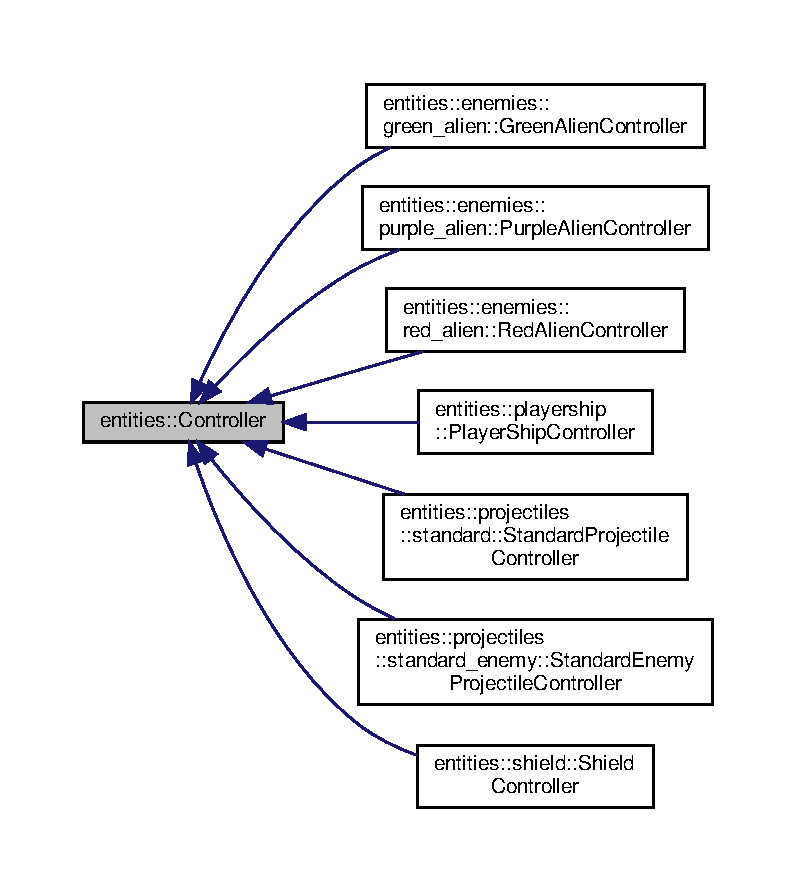
\includegraphics[width=350pt]{classentities_1_1Controller__inherit__graph}
\end{center}
\end{figure}


Collaboration diagram for entities\+:\+:Controller\+:\nopagebreak
\begin{figure}[H]
\begin{center}
\leavevmode
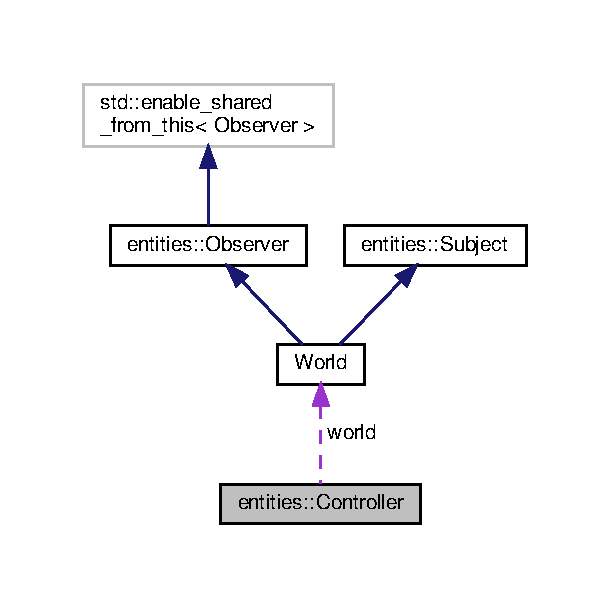
\includegraphics[width=293pt]{classentities_1_1Controller__coll__graph}
\end{center}
\end{figure}
\subsection*{Public Member Functions}
\begin{DoxyCompactItemize}
\item 
\mbox{\Hypertarget{classentities_1_1Controller_ab13d103795b6d18dff0849e94c043e3f}\label{classentities_1_1Controller_ab13d103795b6d18dff0849e94c043e3f}} 
{\bfseries Controller} (\hyperlink{classWorld}{World} \&world, std\+::shared\+\_\+ptr$<$ \hyperlink{classentities_1_1Entity}{Entity} $>$ entity, std\+::shared\+\_\+ptr$<$ \hyperlink{classentities_1_1View}{View} $>$ view)
\item 
\mbox{\Hypertarget{classentities_1_1Controller_a8e92d8a8e3b215295708a4cf25abcf4f}\label{classentities_1_1Controller_a8e92d8a8e3b215295708a4cf25abcf4f}} 
virtual bool {\bfseries handle\+Events} (const std\+::vector$<$ std\+::shared\+\_\+ptr$<$ \hyperlink{classentities_1_1Entity}{Entity} $>$$>$ \&entities)=0
\end{DoxyCompactItemize}
\subsection*{Protected Attributes}
\begin{DoxyCompactItemize}
\item 
\mbox{\Hypertarget{classentities_1_1Controller_a6490e859b0c6d8e96ecc46d68585a81e}\label{classentities_1_1Controller_a6490e859b0c6d8e96ecc46d68585a81e}} 
\hyperlink{classWorld}{World} \& {\bfseries world}
\item 
\mbox{\Hypertarget{classentities_1_1Controller_af114a0e2ca717f637b518c25bfa0c89a}\label{classentities_1_1Controller_af114a0e2ca717f637b518c25bfa0c89a}} 
std\+::shared\+\_\+ptr$<$ \hyperlink{classentities_1_1Entity}{Entity} $>$ {\bfseries entity}
\item 
\mbox{\Hypertarget{classentities_1_1Controller_a8af4452aef4ef06e9798889fca6ea48d}\label{classentities_1_1Controller_a8af4452aef4ef06e9798889fca6ea48d}} 
std\+::shared\+\_\+ptr$<$ \hyperlink{classentities_1_1View}{View} $>$ {\bfseries view}
\end{DoxyCompactItemize}


The documentation for this class was generated from the following file\+:\begin{DoxyCompactItemize}
\item 
/home/mano/\+Documents/univ/space\+\_\+invaders/src/entities/abstract\+\_\+classes/\hyperlink{Controller_8h}{Controller.\+h}\end{DoxyCompactItemize}

\hypertarget{classobjects_1_1enemies_1_1Enemy}{}\section{objects\+:\+:enemies\+:\+:Enemy Class Reference}
\label{classobjects_1_1enemies_1_1Enemy}\index{objects\+::enemies\+::\+Enemy@{objects\+::enemies\+::\+Enemy}}


Inheritance diagram for objects\+:\+:enemies\+:\+:Enemy\+:\nopagebreak
\begin{figure}[H]
\begin{center}
\leavevmode
\includegraphics[width=350pt]{classobjects_1_1enemies_1_1Enemy__inherit__graph}
\end{center}
\end{figure}


Collaboration diagram for objects\+:\+:enemies\+:\+:Enemy\+:\nopagebreak
\begin{figure}[H]
\begin{center}
\leavevmode
\includegraphics[width=177pt]{classobjects_1_1enemies_1_1Enemy__coll__graph}
\end{center}
\end{figure}
\subsection*{Public Member Functions}
\begin{DoxyCompactItemize}
\item 
\mbox{\Hypertarget{classobjects_1_1enemies_1_1Enemy_a0e3ad09de3d7cc19e5f01dd4d9424ee8}\label{classobjects_1_1enemies_1_1Enemy_a0e3ad09de3d7cc19e5f01dd4d9424ee8}}
{\bfseries Enemy} (float x, float y)
\item 
\mbox{\Hypertarget{classobjects_1_1enemies_1_1Enemy_a9a398f8d12234f02563b27440aff7891}\label{classobjects_1_1enemies_1_1Enemy_a9a398f8d12234f02563b27440aff7891}}
virtual void {\bfseries move} ()
\item 
\mbox{\Hypertarget{classobjects_1_1enemies_1_1Enemy_ae89eefd8e9478d7e4512bc24ca52a4b1}\label{classobjects_1_1enemies_1_1Enemy_ae89eefd8e9478d7e4512bc24ca52a4b1}}
virtual void {\bfseries take\+Damage} (float damage)
\end{DoxyCompactItemize}
\subsection*{Public Attributes}
\begin{DoxyCompactItemize}
\item 
\mbox{\Hypertarget{classobjects_1_1enemies_1_1Enemy_abb65eb4904db5b17e78037baba8c42e5}\label{classobjects_1_1enemies_1_1Enemy_abb65eb4904db5b17e78037baba8c42e5}}
float {\bfseries hitpoints}
\end{DoxyCompactItemize}
\subsection*{Protected Attributes}
\begin{DoxyCompactItemize}
\item 
\mbox{\Hypertarget{classobjects_1_1enemies_1_1Enemy_a2721c1375a8a67c1cb6e0c1bd5145b79}\label{classobjects_1_1enemies_1_1Enemy_a2721c1375a8a67c1cb6e0c1bd5145b79}}
const float {\bfseries vspeed}
\item 
\mbox{\Hypertarget{classobjects_1_1enemies_1_1Enemy_a71523230e1a995495e1079bd800101ca}\label{classobjects_1_1enemies_1_1Enemy_a71523230e1a995495e1079bd800101ca}}
const float {\bfseries hspeed}
\item 
\mbox{\Hypertarget{classobjects_1_1enemies_1_1Enemy_a3e48faf63338b8dd57de1b197f1c4159}\label{classobjects_1_1enemies_1_1Enemy_a3e48faf63338b8dd57de1b197f1c4159}}
float {\bfseries dir}
\item 
\mbox{\Hypertarget{classobjects_1_1enemies_1_1Enemy_a798310404e04fa3a626f9307e83e7362}\label{classobjects_1_1enemies_1_1Enemy_a798310404e04fa3a626f9307e83e7362}}
int {\bfseries count}
\item 
\mbox{\Hypertarget{classobjects_1_1enemies_1_1Enemy_ac930ca52dbc7affbd340eaac5b2a2b61}\label{classobjects_1_1enemies_1_1Enemy_ac930ca52dbc7affbd340eaac5b2a2b61}}
bool {\bfseries vertical}
\end{DoxyCompactItemize}
\subsection*{Additional Inherited Members}


The documentation for this class was generated from the following files\+:\begin{DoxyCompactItemize}
\item 
/home/mano/\+Documents/univ/space\+\_\+invaders/src/objects/enemies/\hyperlink{Enemy_8h}{Enemy.\+h}\item
/home/mano/\+Documents/univ/space\+\_\+invaders/src/objects/enemies/\hyperlink{Enemy_8cpp}{Enemy.\+cpp}\end{DoxyCompactItemize}

\hypertarget{classentities_1_1Entity}{}\section{entities\+:\+:Entity Class Reference}
\label{classentities_1_1Entity}\index{entities\+::\+Entity@{entities\+::\+Entity}}


Inheritance diagram for entities\+:\+:Entity\+:\nopagebreak
\begin{figure}[H]
\begin{center}
\leavevmode
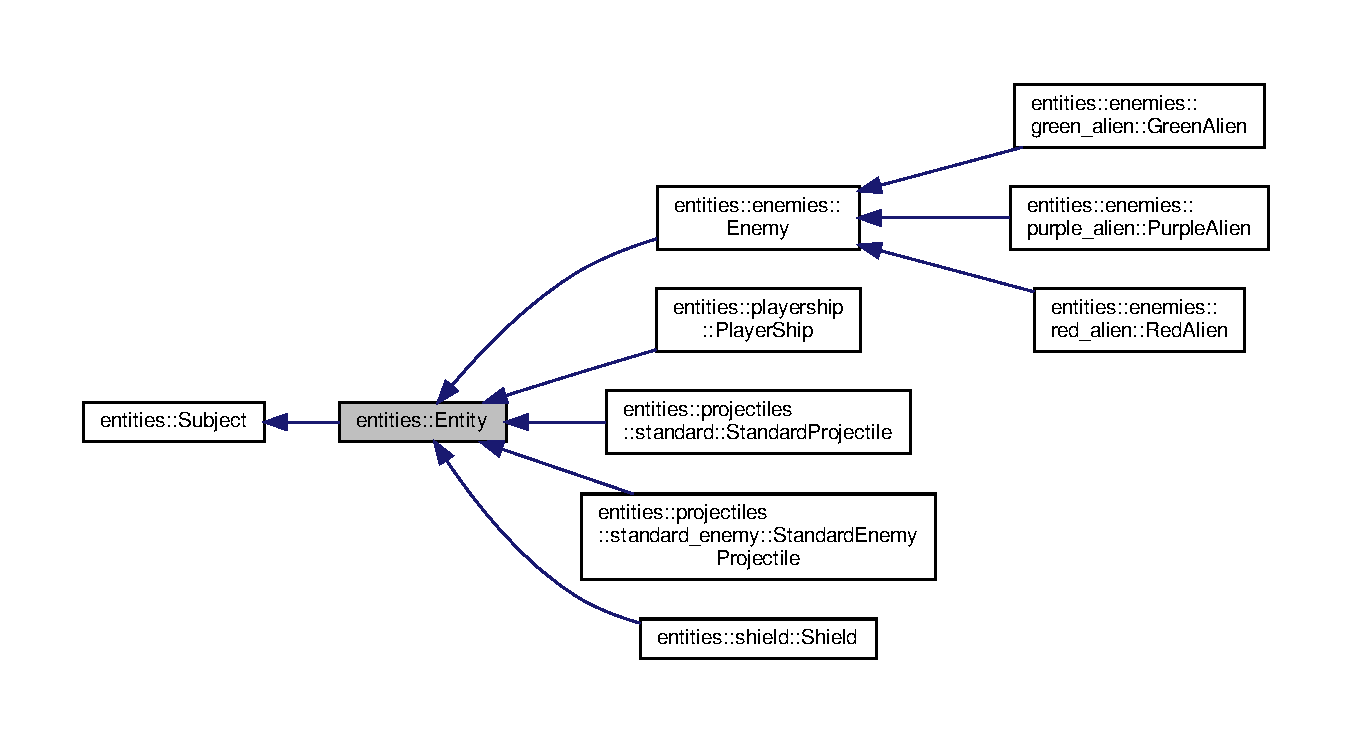
\includegraphics[width=350pt]{classentities_1_1Entity__inherit__graph}
\end{center}
\end{figure}


Collaboration diagram for entities\+:\+:Entity\+:\nopagebreak
\begin{figure}[H]
\begin{center}
\leavevmode
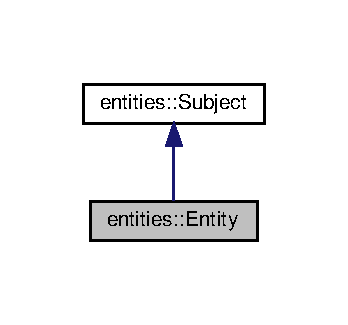
\includegraphics[width=167pt]{classentities_1_1Entity__coll__graph}
\end{center}
\end{figure}
\subsection*{Public Member Functions}
\begin{DoxyCompactItemize}
\item 
\mbox{\Hypertarget{classentities_1_1Entity_a3296f5835063af13ba9569156389f0dc}\label{classentities_1_1Entity_a3296f5835063af13ba9569156389f0dc}} 
{\bfseries Entity} (float x, float y)
\item 
\mbox{\Hypertarget{classentities_1_1Entity_a691e01bec14ee30f0dafbc737c91dd65}\label{classentities_1_1Entity_a691e01bec14ee30f0dafbc737c91dd65}} 
virtual void {\bfseries update} ()=0
\item 
\mbox{\Hypertarget{classentities_1_1Entity_a2c862fc18b3bfbdc0be17c1a3aaf481e}\label{classentities_1_1Entity_a2c862fc18b3bfbdc0be17c1a3aaf481e}} 
float {\bfseries getX} () const
\item 
\mbox{\Hypertarget{classentities_1_1Entity_aca6bc17b74cb9f128c7d2dcc35289872}\label{classentities_1_1Entity_aca6bc17b74cb9f128c7d2dcc35289872}} 
float {\bfseries getY} () const
\item 
\mbox{\Hypertarget{classentities_1_1Entity_a39f898fbcc8567863445b4eb37cd0c8e}\label{classentities_1_1Entity_a39f898fbcc8567863445b4eb37cd0c8e}} 
float {\bfseries get\+X\+Size} () const
\item 
\mbox{\Hypertarget{classentities_1_1Entity_ac2d2d809988105028e4780ca9ae7bef0}\label{classentities_1_1Entity_ac2d2d809988105028e4780ca9ae7bef0}} 
float {\bfseries get\+Y\+Size} () const
\item 
\mbox{\Hypertarget{classentities_1_1Entity_aa3a8d8b0fe6c9d24ceefc2ee9b43eeba}\label{classentities_1_1Entity_aa3a8d8b0fe6c9d24ceefc2ee9b43eeba}} 
void {\bfseries set\+X\+Size} (float x\+Size)
\item 
\mbox{\Hypertarget{classentities_1_1Entity_a84bfd5b99f29a311ba56d2a169159a58}\label{classentities_1_1Entity_a84bfd5b99f29a311ba56d2a169159a58}} 
void {\bfseries set\+Y\+Size} (float y\+Size)
\end{DoxyCompactItemize}
\subsection*{Protected Attributes}
\begin{DoxyCompactItemize}
\item 
\mbox{\Hypertarget{classentities_1_1Entity_a5f6bfef09f32ec0318c4e9b31f3f5d30}\label{classentities_1_1Entity_a5f6bfef09f32ec0318c4e9b31f3f5d30}} 
float {\bfseries x}
\item 
\mbox{\Hypertarget{classentities_1_1Entity_ad86552a73f78657191886938a112650d}\label{classentities_1_1Entity_ad86552a73f78657191886938a112650d}} 
float {\bfseries y}
\item 
\mbox{\Hypertarget{classentities_1_1Entity_a6c6229b1adff361f2417be10f9c40f9e}\label{classentities_1_1Entity_a6c6229b1adff361f2417be10f9c40f9e}} 
float {\bfseries x\+Size} \{\}
\item 
\mbox{\Hypertarget{classentities_1_1Entity_a62e94bd59fe6248b0e1d61e470d7b2b7}\label{classentities_1_1Entity_a62e94bd59fe6248b0e1d61e470d7b2b7}} 
float {\bfseries y\+Size} \{\}
\end{DoxyCompactItemize}
\subsection*{Additional Inherited Members}


The documentation for this class was generated from the following file\+:\begin{DoxyCompactItemize}
\item 
/home/mano/\+Documents/univ/space\+\_\+invaders/src/entities/abstract\+\_\+classes/\hyperlink{Entity_8h}{Entity.\+h}\end{DoxyCompactItemize}

\hypertarget{classGame}{}\section{Game Class Reference}
\label{classGame}\index{Game@{Game}}
\subsection*{Public Member Functions}
\begin{DoxyCompactItemize}
\item 
\hyperlink{classGame_ae84079995ee22675be0adfbaa54940d9}{Game} (const std\+::string \&settings)
\item 
void \hyperlink{classGame_a36587df95a3343658a2d02674050abd7}{play\+Levels} ()
\end{DoxyCompactItemize}


\subsection{Constructor \& Destructor Documentation}
\mbox{\Hypertarget{classGame_ae84079995ee22675be0adfbaa54940d9}\label{classGame_ae84079995ee22675be0adfbaa54940d9}} 
\index{Game@{Game}!Game@{Game}}
\index{Game@{Game}!Game@{Game}}
\subsubsection{\texorpdfstring{Game()}{Game()}}
{\footnotesize\ttfamily Game\+::\+Game (\begin{DoxyParamCaption}\item[{const std\+::string \&}]{settings }\end{DoxyParamCaption})\hspace{0.3cm}{\ttfamily [explicit]}}


\begin{DoxyParams}{Parameters}
{\em settings} & a json file containing the game settings \\
\hline
\end{DoxyParams}


\subsection{Member Function Documentation}
\mbox{\Hypertarget{classGame_a36587df95a3343658a2d02674050abd7}\label{classGame_a36587df95a3343658a2d02674050abd7}} 
\index{Game@{Game}!play\+Levels@{play\+Levels}}
\index{play\+Levels@{play\+Levels}!Game@{Game}}
\subsubsection{\texorpdfstring{play\+Levels()}{playLevels()}}
{\footnotesize\ttfamily void Game\+::play\+Levels (\begin{DoxyParamCaption}{ }\end{DoxyParamCaption})}

starts playing all the levels described in the settings file 

The documentation for this class was generated from the following files\+:\begin{DoxyCompactItemize}
\item 
/home/mano/\+Documents/univ/space\+\_\+invaders/src/game/\hyperlink{Game_8h}{Game.\+h}\item 
/home/mano/\+Documents/univ/space\+\_\+invaders/src/game/Game.\+cpp\item 
/home/mano/\+Documents/univ/space\+\_\+invaders/src/game/Game\+Screens.\+cpp\end{DoxyCompactItemize}

\hypertarget{classobjects_1_1enemies_1_1green__alien_1_1GreenAlien}{}\section{objects\+:\+:enemies\+:\+:green\+\_\+alien\+:\+:Green\+Alien Class Reference}
\label{classobjects_1_1enemies_1_1green__alien_1_1GreenAlien}\index{objects\+::enemies\+::green\+\_\+alien\+::\+Green\+Alien@{objects\+::enemies\+::green\+\_\+alien\+::\+Green\+Alien}}


Inheritance diagram for objects\+:\+:enemies\+:\+:green\+\_\+alien\+:\+:Green\+Alien\+:\nopagebreak
\begin{figure}[H]
\begin{center}
\leavevmode
\includegraphics[width=200pt]{classobjects_1_1enemies_1_1green__alien_1_1GreenAlien__inherit__graph}
\end{center}
\end{figure}


Collaboration diagram for objects\+:\+:enemies\+:\+:green\+\_\+alien\+:\+:Green\+Alien\+:\nopagebreak
\begin{figure}[H]
\begin{center}
\leavevmode
\includegraphics[width=200pt]{classobjects_1_1enemies_1_1green__alien_1_1GreenAlien__coll__graph}
\end{center}
\end{figure}
\subsection*{Public Member Functions}
\begin{DoxyCompactItemize}
\item 
\mbox{\Hypertarget{classobjects_1_1enemies_1_1green__alien_1_1GreenAlien_a77d12c28dac45b2ffacfa717ea32f139}\label{classobjects_1_1enemies_1_1green__alien_1_1GreenAlien_a77d12c28dac45b2ffacfa717ea32f139}}
{\bfseries Green\+Alien} (float x, float y)
\item 
\mbox{\Hypertarget{classobjects_1_1enemies_1_1green__alien_1_1GreenAlien_a8489bee31c00c660f067172a97d3121d}\label{classobjects_1_1enemies_1_1green__alien_1_1GreenAlien_a8489bee31c00c660f067172a97d3121d}}
void {\bfseries update} () override
\end{DoxyCompactItemize}
\subsection*{Additional Inherited Members}


The documentation for this class was generated from the following files\+:\begin{DoxyCompactItemize}
\item 
/home/mano/\+Documents/univ/space\+\_\+invaders/src/objects/enemies/green\+\_\+alien/\hyperlink{GreenAlien_8h}{Green\+Alien.\+h}\item
/home/mano/\+Documents/univ/space\+\_\+invaders/src/objects/enemies/green\+\_\+alien/\hyperlink{GreenAlien_8cpp}{Green\+Alien.\+cpp}\end{DoxyCompactItemize}

\hypertarget{classobjects_1_1enemies_1_1green__alien_1_1GreenAlienController}{}\section{objects\+:\+:enemies\+:\+:green\+\_\+alien\+:\+:Green\+Alien\+Controller Class Reference}
\label{classobjects_1_1enemies_1_1green__alien_1_1GreenAlienController}\index{objects\+::enemies\+::green\+\_\+alien\+::\+Green\+Alien\+Controller@{objects\+::enemies\+::green\+\_\+alien\+::\+Green\+Alien\+Controller}}


Inheritance diagram for objects\+:\+:enemies\+:\+:green\+\_\+alien\+:\+:Green\+Alien\+Controller\+:\nopagebreak
\begin{figure}[H]
\begin{center}
\leavevmode
\includegraphics[width=242pt]{classobjects_1_1enemies_1_1green__alien_1_1GreenAlienController__inherit__graph}
\end{center}
\end{figure}


Collaboration diagram for objects\+:\+:enemies\+:\+:green\+\_\+alien\+:\+:Green\+Alien\+Controller\+:\nopagebreak
\begin{figure}[H]
\begin{center}
\leavevmode
\includegraphics[width=293pt]{classobjects_1_1enemies_1_1green__alien_1_1GreenAlienController__coll__graph}
\end{center}
\end{figure}
\subsection*{Public Member Functions}
\begin{DoxyCompactItemize}
\item 
\mbox{\Hypertarget{classobjects_1_1enemies_1_1green__alien_1_1GreenAlienController_af175899c90308195285ff3e7db10c9df}\label{classobjects_1_1enemies_1_1green__alien_1_1GreenAlienController_af175899c90308195285ff3e7db10c9df}}
{\bfseries Green\+Alien\+Controller} (const std\+::shared\+\_\+ptr$<$ \hyperlink{classobjects_1_1Entity}{Entity} $>$ \&entity, const std\+::shared\+\_\+ptr$<$ \hyperlink{classobjects_1_1View}{View} $>$ \&view, \hyperlink{classWorld}{World} \&world)
\item 
\mbox{\Hypertarget{classobjects_1_1enemies_1_1green__alien_1_1GreenAlienController_a63fb5ef2420687dd3dc37412a13f9c8e}\label{classobjects_1_1enemies_1_1green__alien_1_1GreenAlienController_a63fb5ef2420687dd3dc37412a13f9c8e}}
bool {\bfseries handle\+Events} (const std\+::vector$<$ std\+::shared\+\_\+ptr$<$ \hyperlink{classobjects_1_1Entity}{Entity} $>$$>$ \&objects) override
\end{DoxyCompactItemize}
\subsection*{Additional Inherited Members}


The documentation for this class was generated from the following files\+:\begin{DoxyCompactItemize}
\item 
/home/mano/\+Documents/univ/space\+\_\+invaders/src/objects/enemies/green\+\_\+alien/\hyperlink{GreenAlienController_8h}{Green\+Alien\+Controller.\+h}\item
/home/mano/\+Documents/univ/space\+\_\+invaders/src/objects/enemies/green\+\_\+alien/\hyperlink{GreenAlienController_8cpp}{Green\+Alien\+Controller.\+cpp}\end{DoxyCompactItemize}

\hypertarget{classentities_1_1enemies_1_1green__alien_1_1GreenAlienView}{}\section{entities\+:\+:enemies\+:\+:green\+\_\+alien\+:\+:Green\+Alien\+View Class Reference}
\label{classentities_1_1enemies_1_1green__alien_1_1GreenAlienView}\index{entities\+::enemies\+::green\+\_\+alien\+::\+Green\+Alien\+View@{entities\+::enemies\+::green\+\_\+alien\+::\+Green\+Alien\+View}}


Inheritance diagram for entities\+:\+:enemies\+:\+:green\+\_\+alien\+:\+:Green\+Alien\+View\+:\nopagebreak
\begin{figure}[H]
\begin{center}
\leavevmode
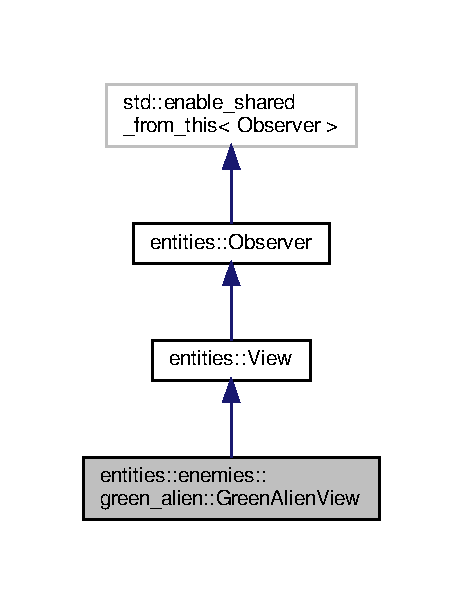
\includegraphics[width=222pt]{classentities_1_1enemies_1_1green__alien_1_1GreenAlienView__inherit__graph}
\end{center}
\end{figure}


Collaboration diagram for entities\+:\+:enemies\+:\+:green\+\_\+alien\+:\+:Green\+Alien\+View\+:\nopagebreak
\begin{figure}[H]
\begin{center}
\leavevmode
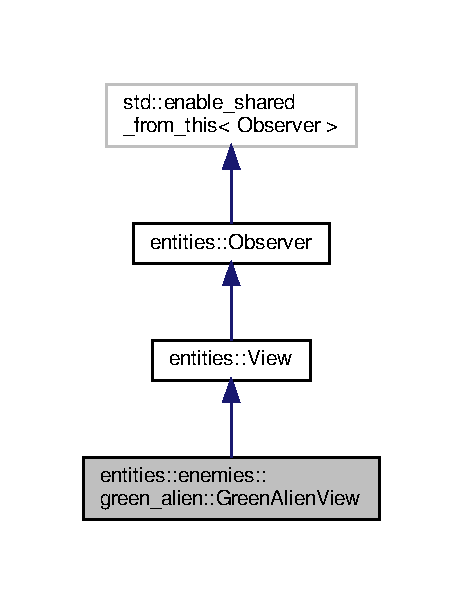
\includegraphics[width=222pt]{classentities_1_1enemies_1_1green__alien_1_1GreenAlienView__coll__graph}
\end{center}
\end{figure}
\subsection*{Public Member Functions}
\begin{DoxyCompactItemize}
\item 
\mbox{\Hypertarget{classentities_1_1enemies_1_1green__alien_1_1GreenAlienView_a3db2841587821504e4073cef87cf7dc1}\label{classentities_1_1enemies_1_1green__alien_1_1GreenAlienView_a3db2841587821504e4073cef87cf7dc1}} 
{\bfseries Green\+Alien\+View} (const std\+::shared\+\_\+ptr$<$ \hyperlink{classentities_1_1enemies_1_1green__alien_1_1GreenAlien}{Green\+Alien} $>$ \&alien)
\item 
\mbox{\Hypertarget{classentities_1_1enemies_1_1green__alien_1_1GreenAlienView_a18e2193d589d73e6449b14bfe2e2e99e}\label{classentities_1_1enemies_1_1green__alien_1_1GreenAlienView_a18e2193d589d73e6449b14bfe2e2e99e}} 
void {\bfseries on\+Notify} () override
\end{DoxyCompactItemize}
\subsection*{Additional Inherited Members}


The documentation for this class was generated from the following files\+:\begin{DoxyCompactItemize}
\item 
/home/mano/\+Documents/univ/space\+\_\+invaders/src/entities/enemies/green\+\_\+alien/\hyperlink{GreenAlienView_8h}{Green\+Alien\+View.\+h}\item 
/home/mano/\+Documents/univ/space\+\_\+invaders/src/entities/enemies/green\+\_\+alien/\hyperlink{GreenAlienView_8cpp}{Green\+Alien\+View.\+cpp}\end{DoxyCompactItemize}

\hypertarget{classentities_1_1Observer}{}\section{entities\+:\+:Observer Class Reference}
\label{classentities_1_1Observer}\index{entities\+::\+Observer@{entities\+::\+Observer}}


Inheritance diagram for entities\+:\+:Observer\+:\nopagebreak
\begin{figure}[H]
\begin{center}
\leavevmode
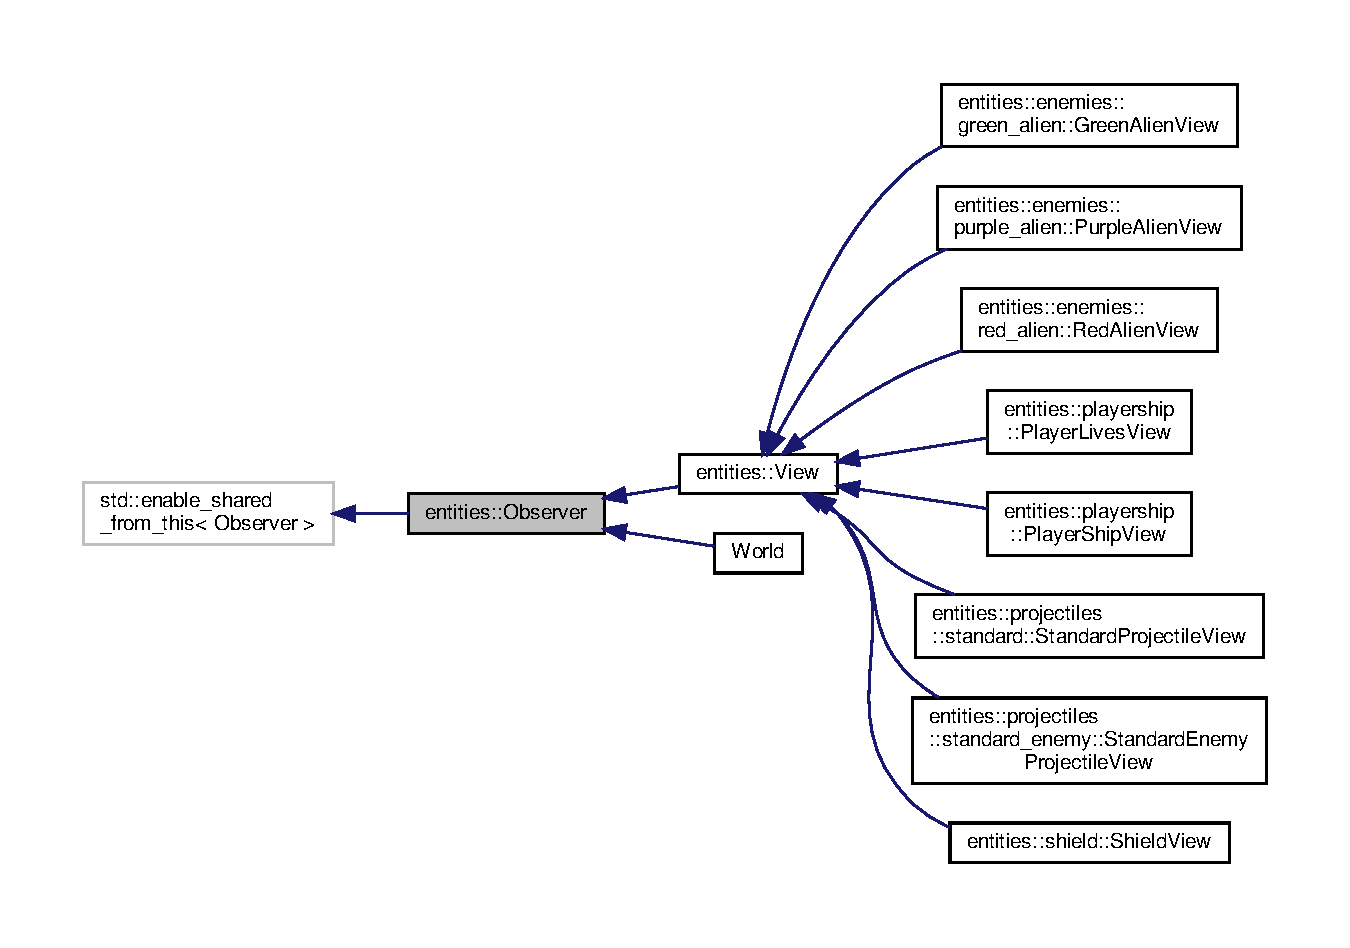
\includegraphics[width=350pt]{classentities_1_1Observer__inherit__graph}
\end{center}
\end{figure}


Collaboration diagram for entities\+:\+:Observer\+:\nopagebreak
\begin{figure}[H]
\begin{center}
\leavevmode
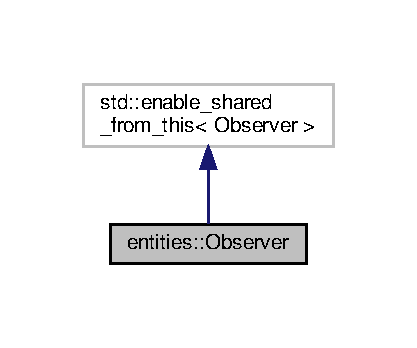
\includegraphics[width=200pt]{classentities_1_1Observer__coll__graph}
\end{center}
\end{figure}
\subsection*{Public Member Functions}
\begin{DoxyCompactItemize}
\item 
\mbox{\Hypertarget{classentities_1_1Observer_a6c3561b7219abd0f4de7e21e52a899b8}\label{classentities_1_1Observer_a6c3561b7219abd0f4de7e21e52a899b8}} 
virtual void {\bfseries on\+Notify} ()=0
\end{DoxyCompactItemize}


The documentation for this class was generated from the following file\+:\begin{DoxyCompactItemize}
\item 
/home/mano/\+Documents/univ/space\+\_\+invaders/src/entities/abstract\+\_\+classes/\hyperlink{Observer_8h}{Observer.\+h}\end{DoxyCompactItemize}

\hypertarget{classentities_1_1playership_1_1PlayerLivesView}{}\section{entities\+:\+:playership\+:\+:Player\+Lives\+View Class Reference}
\label{classentities_1_1playership_1_1PlayerLivesView}\index{entities\+::playership\+::\+Player\+Lives\+View@{entities\+::playership\+::\+Player\+Lives\+View}}


Inheritance diagram for entities\+:\+:playership\+:\+:Player\+Lives\+View\+:\nopagebreak
\begin{figure}[H]
\begin{center}
\leavevmode
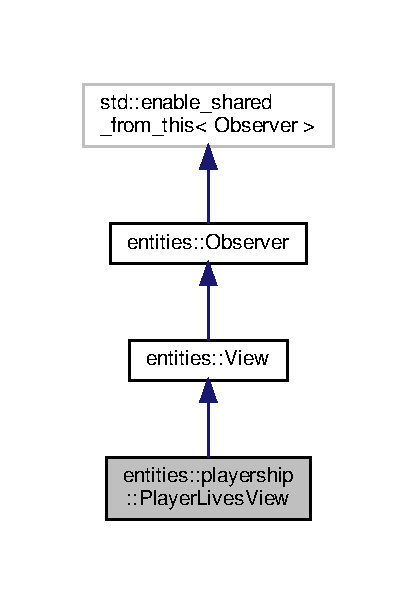
\includegraphics[width=200pt]{classentities_1_1playership_1_1PlayerLivesView__inherit__graph}
\end{center}
\end{figure}


Collaboration diagram for entities\+:\+:playership\+:\+:Player\+Lives\+View\+:\nopagebreak
\begin{figure}[H]
\begin{center}
\leavevmode
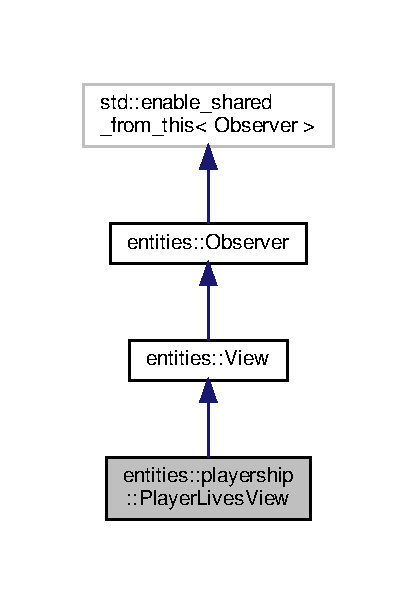
\includegraphics[width=200pt]{classentities_1_1playership_1_1PlayerLivesView__coll__graph}
\end{center}
\end{figure}
\subsection*{Public Member Functions}
\begin{DoxyCompactItemize}
\item 
\mbox{\Hypertarget{classentities_1_1playership_1_1PlayerLivesView_a3641cc3d57cd2d39c239ccf55bbf753b}\label{classentities_1_1playership_1_1PlayerLivesView_a3641cc3d57cd2d39c239ccf55bbf753b}} 
{\bfseries Player\+Lives\+View} (std\+::shared\+\_\+ptr$<$ \hyperlink{classentities_1_1playership_1_1PlayerShip}{Player\+Ship} $>$ ship)
\item 
\mbox{\Hypertarget{classentities_1_1playership_1_1PlayerLivesView_acb60896fe7d67a869173161c3df8221c}\label{classentities_1_1playership_1_1PlayerLivesView_acb60896fe7d67a869173161c3df8221c}} 
void {\bfseries on\+Notify} () override
\item 
\mbox{\Hypertarget{classentities_1_1playership_1_1PlayerLivesView_afda45f04f11cb8e76b9de1595b0feceb}\label{classentities_1_1playership_1_1PlayerLivesView_afda45f04f11cb8e76b9de1595b0feceb}} 
void {\bfseries draw} (sf\+::\+Render\+Window \&window) const override
\end{DoxyCompactItemize}
\subsection*{Additional Inherited Members}


The documentation for this class was generated from the following files\+:\begin{DoxyCompactItemize}
\item 
/home/mano/\+Documents/univ/space\+\_\+invaders/src/entities/playership/\hyperlink{PlayerLivesView_8h}{Player\+Lives\+View.\+h}\item 
/home/mano/\+Documents/univ/space\+\_\+invaders/src/entities/playership/\hyperlink{PlayerLivesView_8cpp}{Player\+Lives\+View.\+cpp}\end{DoxyCompactItemize}

\hypertarget{classobjects_1_1playership_1_1PlayerShip}{}\section{objects\+:\+:playership\+:\+:Player\+Ship Class Reference}
\label{classobjects_1_1playership_1_1PlayerShip}\index{objects\+::playership\+::\+Player\+Ship@{objects\+::playership\+::\+Player\+Ship}}


Inheritance diagram for objects\+:\+:playership\+:\+:Player\+Ship\+:\nopagebreak
\begin{figure}[H]
\begin{center}
\leavevmode
\includegraphics[width=178pt]{classobjects_1_1playership_1_1PlayerShip__inherit__graph}
\end{center}
\end{figure}


Collaboration diagram for objects\+:\+:playership\+:\+:Player\+Ship\+:\nopagebreak
\begin{figure}[H]
\begin{center}
\leavevmode
\includegraphics[width=178pt]{classobjects_1_1playership_1_1PlayerShip__coll__graph}
\end{center}
\end{figure}
\subsection*{Public Member Functions}
\begin{DoxyCompactItemize}
\item 
\mbox{\Hypertarget{classobjects_1_1playership_1_1PlayerShip_a17a64b5b78b9fa9c06601634d527ef77}\label{classobjects_1_1playership_1_1PlayerShip_a17a64b5b78b9fa9c06601634d527ef77}}
{\bfseries Player\+Ship} (float x, float y)
\item 
\mbox{\Hypertarget{classobjects_1_1playership_1_1PlayerShip_ae1855813ac0cfde9be1d9dfbf307f72e}\label{classobjects_1_1playership_1_1PlayerShip_ae1855813ac0cfde9be1d9dfbf307f72e}}
void {\bfseries move\+Left} ()
\item 
\mbox{\Hypertarget{classobjects_1_1playership_1_1PlayerShip_a9708f989ced14f082c36051e8a9710f7}\label{classobjects_1_1playership_1_1PlayerShip_a9708f989ced14f082c36051e8a9710f7}}
void {\bfseries move\+Right} ()
\item 
\mbox{\Hypertarget{classobjects_1_1playership_1_1PlayerShip_a0fdd05020563087b024831c93dad8ee1}\label{classobjects_1_1playership_1_1PlayerShip_a0fdd05020563087b024831c93dad8ee1}}
void {\bfseries take\+Damage} (float damage)
\item 
\mbox{\Hypertarget{classobjects_1_1playership_1_1PlayerShip_a618c1a8fd743a8fcbe9e60b44bd21dca}\label{classobjects_1_1playership_1_1PlayerShip_a618c1a8fd743a8fcbe9e60b44bd21dca}}
void {\bfseries update} () override
\end{DoxyCompactItemize}
\subsection*{Public Attributes}
\begin{DoxyCompactItemize}
\item 
\mbox{\Hypertarget{classobjects_1_1playership_1_1PlayerShip_ab9cf9712f43739b1ba9d6b83ae45fd4c}\label{classobjects_1_1playership_1_1PlayerShip_ab9cf9712f43739b1ba9d6b83ae45fd4c}}
float {\bfseries hitpoints}
\end{DoxyCompactItemize}
\subsection*{Additional Inherited Members}


The documentation for this class was generated from the following files\+:\begin{DoxyCompactItemize}
\item 
/home/mano/\+Documents/univ/space\+\_\+invaders/src/objects/playership/\hyperlink{PlayerShip_8h}{Player\+Ship.\+h}\item
/home/mano/\+Documents/univ/space\+\_\+invaders/src/objects/playership/\hyperlink{PlayerShip_8cpp}{Player\+Ship.\+cpp}\end{DoxyCompactItemize}

\hypertarget{classentities_1_1playership_1_1PlayerShipController}{}\section{entities\+:\+:playership\+:\+:Player\+Ship\+Controller Class Reference}
\label{classentities_1_1playership_1_1PlayerShipController}\index{entities\+::playership\+::\+Player\+Ship\+Controller@{entities\+::playership\+::\+Player\+Ship\+Controller}}


Inheritance diagram for entities\+:\+:playership\+:\+:Player\+Ship\+Controller\+:\nopagebreak
\begin{figure}[H]
\begin{center}
\leavevmode
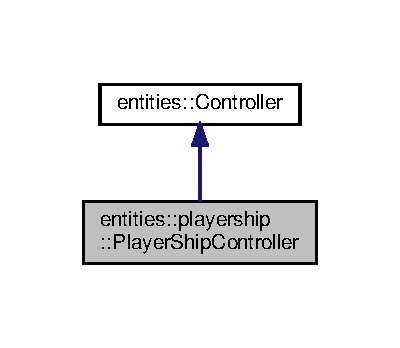
\includegraphics[width=192pt]{classentities_1_1playership_1_1PlayerShipController__inherit__graph}
\end{center}
\end{figure}


Collaboration diagram for entities\+:\+:playership\+:\+:Player\+Ship\+Controller\+:\nopagebreak
\begin{figure}[H]
\begin{center}
\leavevmode
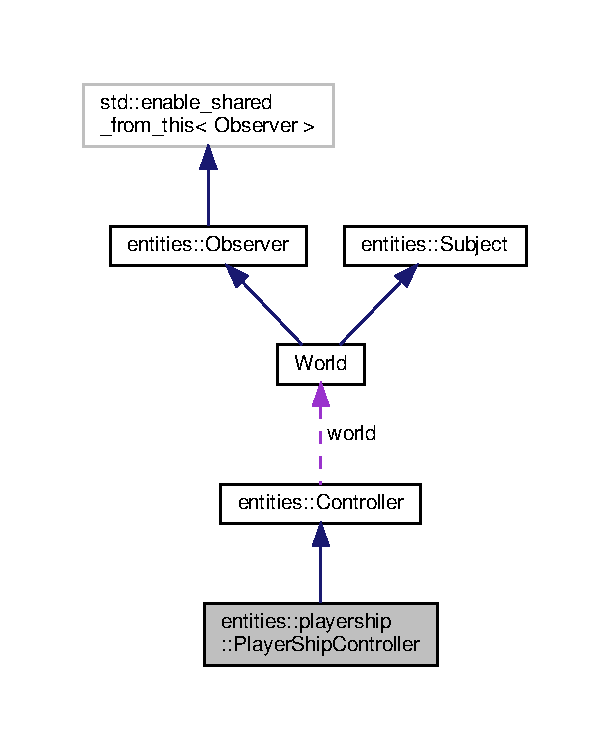
\includegraphics[width=293pt]{classentities_1_1playership_1_1PlayerShipController__coll__graph}
\end{center}
\end{figure}
\subsection*{Public Member Functions}
\begin{DoxyCompactItemize}
\item 
\mbox{\Hypertarget{classentities_1_1playership_1_1PlayerShipController_a5f57a0601302205580b099c4037ab2d7}\label{classentities_1_1playership_1_1PlayerShipController_a5f57a0601302205580b099c4037ab2d7}} 
{\bfseries Player\+Ship\+Controller} (const std\+::shared\+\_\+ptr$<$ \hyperlink{classentities_1_1Entity}{Entity} $>$ \&entity, const std\+::shared\+\_\+ptr$<$ \hyperlink{classentities_1_1View}{View} $>$ \&view, \hyperlink{classWorld}{World} \&world)
\item 
\mbox{\Hypertarget{classentities_1_1playership_1_1PlayerShipController_ad3af27cacdd1e761b9ae2fab78814325}\label{classentities_1_1playership_1_1PlayerShipController_ad3af27cacdd1e761b9ae2fab78814325}} 
bool {\bfseries handle\+Events} (const std\+::vector$<$ std\+::shared\+\_\+ptr$<$ \hyperlink{classentities_1_1Entity}{Entity} $>$$>$ \&entities) override
\end{DoxyCompactItemize}
\subsection*{Additional Inherited Members}


The documentation for this class was generated from the following files\+:\begin{DoxyCompactItemize}
\item 
/home/mano/\+Documents/univ/space\+\_\+invaders/src/entities/playership/\hyperlink{PlayerShipController_8h}{Player\+Ship\+Controller.\+h}\item 
/home/mano/\+Documents/univ/space\+\_\+invaders/src/entities/playership/\hyperlink{PlayerShipController_8cpp}{Player\+Ship\+Controller.\+cpp}\end{DoxyCompactItemize}

\hypertarget{classobjects_1_1playership_1_1PlayerShipView}{}\section{objects\+:\+:playership\+:\+:Player\+Ship\+View Class Reference}
\label{classobjects_1_1playership_1_1PlayerShipView}\index{objects\+::playership\+::\+Player\+Ship\+View@{objects\+::playership\+::\+Player\+Ship\+View}}


Inheritance diagram for objects\+:\+:playership\+:\+:Player\+Ship\+View\+:\nopagebreak
\begin{figure}[H]
\begin{center}
\leavevmode
\includegraphics[width=200pt]{classobjects_1_1playership_1_1PlayerShipView__inherit__graph}
\end{center}
\end{figure}


Collaboration diagram for objects\+:\+:playership\+:\+:Player\+Ship\+View\+:\nopagebreak
\begin{figure}[H]
\begin{center}
\leavevmode
\includegraphics[width=200pt]{classobjects_1_1playership_1_1PlayerShipView__coll__graph}
\end{center}
\end{figure}
\subsection*{Public Member Functions}
\begin{DoxyCompactItemize}
\item 
\mbox{\Hypertarget{classobjects_1_1playership_1_1PlayerShipView_a9f863260d81efc4cdfb213af754b5732}\label{classobjects_1_1playership_1_1PlayerShipView_a9f863260d81efc4cdfb213af754b5732}}
{\bfseries Player\+Ship\+View} (std\+::shared\+\_\+ptr$<$ \hyperlink{classobjects_1_1playership_1_1PlayerShip}{Player\+Ship} $>$ ship)
\item 
\mbox{\Hypertarget{classobjects_1_1playership_1_1PlayerShipView_a141c615a79dabf823243993f699cb039}\label{classobjects_1_1playership_1_1PlayerShipView_a141c615a79dabf823243993f699cb039}}
void {\bfseries on\+Notify} () override
\item 
\mbox{\Hypertarget{classobjects_1_1playership_1_1PlayerShipView_abce403c13058a9d56d8a668c4da659af}\label{classobjects_1_1playership_1_1PlayerShipView_abce403c13058a9d56d8a668c4da659af}}
void {\bfseries draw} (sf\+::\+Render\+Window \&window) const override
\end{DoxyCompactItemize}
\subsection*{Additional Inherited Members}


The documentation for this class was generated from the following files\+:\begin{DoxyCompactItemize}
\item 
/home/mano/\+Documents/univ/space\+\_\+invaders/src/objects/playership/\hyperlink{PlayerShipView_8h}{Player\+Ship\+View.\+h}\item
/home/mano/\+Documents/univ/space\+\_\+invaders/src/objects/playership/\hyperlink{PlayerShipView_8cpp}{Player\+Ship\+View.\+cpp}\end{DoxyCompactItemize}

\hypertarget{classobjects_1_1projectiles_1_1ProjectileFactory}{}\section{objects\+:\+:projectiles\+:\+:Projectile\+Factory Class Reference}
\label{classobjects_1_1projectiles_1_1ProjectileFactory}\index{objects\+::projectiles\+::\+Projectile\+Factory@{objects\+::projectiles\+::\+Projectile\+Factory}}
\subsection*{Public Types}
\begin{DoxyCompactItemize}
\item 
enum \hyperlink{classobjects_1_1projectiles_1_1ProjectileFactory_abc75eceeed2dbadc736fb93fd6046698}{Type} \{ {\bfseries Standard},
{\bfseries Fast}, 
{\bfseries Enemy\+Standard}
 \}
\end{DoxyCompactItemize}
\subsection*{Public Member Functions}
\begin{DoxyCompactItemize}
\item 
\mbox{\Hypertarget{classobjects_1_1projectiles_1_1ProjectileFactory_ad198f3f077022468b6bdd2d114c3a969}\label{classobjects_1_1projectiles_1_1ProjectileFactory_ad198f3f077022468b6bdd2d114c3a969}}
{\bfseries Projectile\+Factory} (const \hyperlink{classobjects_1_1projectiles_1_1ProjectileFactory}{Projectile\+Factory} \&copy)=delete
\item 
\mbox{\Hypertarget{classobjects_1_1projectiles_1_1ProjectileFactory_a23c5feb5df880e4cf133f7e9739deda7}\label{classobjects_1_1projectiles_1_1ProjectileFactory_a23c5feb5df880e4cf133f7e9739deda7}}
\hyperlink{classobjects_1_1projectiles_1_1ProjectileFactory}{Projectile\+Factory} \& {\bfseries operator=} (\hyperlink{classobjects_1_1projectiles_1_1ProjectileFactory}{Projectile\+Factory})=delete
\end{DoxyCompactItemize}
\subsection*{Static Public Member Functions}
\begin{DoxyCompactItemize}
\item 
static void \hyperlink{classobjects_1_1projectiles_1_1ProjectileFactory_ae2fdae24114f0a54e474e1cf14eb34d5}{create\+Projectile} (float x, float y, \hyperlink{classobjects_1_1projectiles_1_1ProjectileFactory_abc75eceeed2dbadc736fb93fd6046698}{Type} type, \hyperlink{classWorld}{World} \&world)
\end{DoxyCompactItemize}


\subsection{Member Enumeration Documentation}
\mbox{\Hypertarget{classobjects_1_1projectiles_1_1ProjectileFactory_abc75eceeed2dbadc736fb93fd6046698}\label{classobjects_1_1projectiles_1_1ProjectileFactory_abc75eceeed2dbadc736fb93fd6046698}}
\index{objects\+::projectiles\+::\+Projectile\+Factory@{objects\+::projectiles\+::\+Projectile\+Factory}!Type@{Type}}
\index{Type@{Type}!objects\+::projectiles\+::\+Projectile\+Factory@{objects\+::projectiles\+::\+Projectile\+Factory}}
\subsubsection{\texorpdfstring{Type}{Type}}
{\footnotesize\ttfamily enum \hyperlink{classobjects_1_1projectiles_1_1ProjectileFactory_abc75eceeed2dbadc736fb93fd6046698}{objects\+::projectiles\+::\+Projectile\+Factory\+::\+Type}}

we use this to indicate which type of projectile we want to be created 

\subsection{Member Function Documentation}
\mbox{\Hypertarget{classobjects_1_1projectiles_1_1ProjectileFactory_ae2fdae24114f0a54e474e1cf14eb34d5}\label{classobjects_1_1projectiles_1_1ProjectileFactory_ae2fdae24114f0a54e474e1cf14eb34d5}}
\index{objects\+::projectiles\+::\+Projectile\+Factory@{objects\+::projectiles\+::\+Projectile\+Factory}!create\+Projectile@{create\+Projectile}}
\index{create\+Projectile@{create\+Projectile}!objects\+::projectiles\+::\+Projectile\+Factory@{objects\+::projectiles\+::\+Projectile\+Factory}}
\subsubsection{\texorpdfstring{create\+Projectile()}{createProjectile()}}
{\footnotesize\ttfamily void Projectile\+Factory\+::create\+Projectile (\begin{DoxyParamCaption}\item[{float}]{x,  }\item[{float}]{y,  }\item[{\hyperlink{classobjects_1_1projectiles_1_1ProjectileFactory_abc75eceeed2dbadc736fb93fd6046698}{Type}}]{type,  }\item[{\hyperlink{classWorld}{World} \&}]{world }\end{DoxyParamCaption})\hspace{0.3cm}{\ttfamily [static]}}

creates a projectile 
\begin{DoxyParams}{Parameters}
{\em x} & the x coordinate where it should be created \\
\hline
{\em y} & the y coordinate where it should be created \\
\hline
{\em type} & the type of the projectile that should be created \\
\hline
{\em world} & the world in which it should be created \\
\hline
\end{DoxyParams}


The documentation for this class was generated from the following files\+:\begin{DoxyCompactItemize}
\item 
/home/mano/\+Documents/univ/space\+\_\+invaders/src/objects/projectiles/\hyperlink{ProjectileFactory_8h}{Projectile\+Factory.\+h}\item
/home/mano/\+Documents/univ/space\+\_\+invaders/src/objects/projectiles/\hyperlink{ProjectileFactory_8cpp}{Projectile\+Factory.\+cpp}\end{DoxyCompactItemize}

\hypertarget{classentities_1_1enemies_1_1purple__alien_1_1PurpleAlien}{}\section{entities\+:\+:enemies\+:\+:purple\+\_\+alien\+:\+:Purple\+Alien Class Reference}
\label{classentities_1_1enemies_1_1purple__alien_1_1PurpleAlien}\index{entities\+::enemies\+::purple\+\_\+alien\+::\+Purple\+Alien@{entities\+::enemies\+::purple\+\_\+alien\+::\+Purple\+Alien}}


Inheritance diagram for entities\+:\+:enemies\+:\+:purple\+\_\+alien\+:\+:Purple\+Alien\+:\nopagebreak
\begin{figure}[H]
\begin{center}
\leavevmode
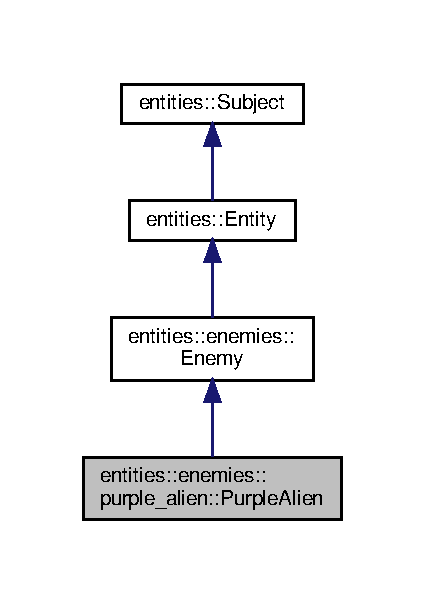
\includegraphics[width=204pt]{classentities_1_1enemies_1_1purple__alien_1_1PurpleAlien__inherit__graph}
\end{center}
\end{figure}


Collaboration diagram for entities\+:\+:enemies\+:\+:purple\+\_\+alien\+:\+:Purple\+Alien\+:\nopagebreak
\begin{figure}[H]
\begin{center}
\leavevmode
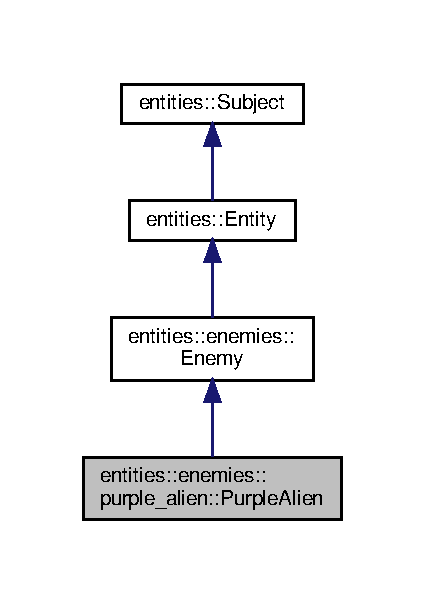
\includegraphics[width=204pt]{classentities_1_1enemies_1_1purple__alien_1_1PurpleAlien__coll__graph}
\end{center}
\end{figure}
\subsection*{Public Member Functions}
\begin{DoxyCompactItemize}
\item 
\mbox{\Hypertarget{classentities_1_1enemies_1_1purple__alien_1_1PurpleAlien_a19496a9f49da18c9c260f98194e695e6}\label{classentities_1_1enemies_1_1purple__alien_1_1PurpleAlien_a19496a9f49da18c9c260f98194e695e6}} 
{\bfseries Purple\+Alien} (float x, float y)
\item 
\mbox{\Hypertarget{classentities_1_1enemies_1_1purple__alien_1_1PurpleAlien_a2e9d3a7d34dc72d7541ccb572b6d5a11}\label{classentities_1_1enemies_1_1purple__alien_1_1PurpleAlien_a2e9d3a7d34dc72d7541ccb572b6d5a11}} 
void {\bfseries update} () override
\end{DoxyCompactItemize}
\subsection*{Public Attributes}
\begin{DoxyCompactItemize}
\item 
\mbox{\Hypertarget{classentities_1_1enemies_1_1purple__alien_1_1PurpleAlien_aacaf3e961373d9ef3a0d05758a811860}\label{classentities_1_1enemies_1_1purple__alien_1_1PurpleAlien_aacaf3e961373d9ef3a0d05758a811860}} 
float {\bfseries max\+Hp}
\end{DoxyCompactItemize}
\subsection*{Additional Inherited Members}


The documentation for this class was generated from the following files\+:\begin{DoxyCompactItemize}
\item 
/home/mano/\+Documents/univ/space\+\_\+invaders/src/entities/enemies/purple\+\_\+alien/\hyperlink{PurpleAlien_8h}{Purple\+Alien.\+h}\item 
/home/mano/\+Documents/univ/space\+\_\+invaders/src/entities/enemies/purple\+\_\+alien/\hyperlink{PurpleAlien_8cpp}{Purple\+Alien.\+cpp}\end{DoxyCompactItemize}

\hypertarget{classentities_1_1enemies_1_1purple__alien_1_1PurpleAlienController}{}\section{entities\+:\+:enemies\+:\+:purple\+\_\+alien\+:\+:Purple\+Alien\+Controller Class Reference}
\label{classentities_1_1enemies_1_1purple__alien_1_1PurpleAlienController}\index{entities\+::enemies\+::purple\+\_\+alien\+::\+Purple\+Alien\+Controller@{entities\+::enemies\+::purple\+\_\+alien\+::\+Purple\+Alien\+Controller}}


Inheritance diagram for entities\+:\+:enemies\+:\+:purple\+\_\+alien\+:\+:Purple\+Alien\+Controller\+:\nopagebreak
\begin{figure}[H]
\begin{center}
\leavevmode
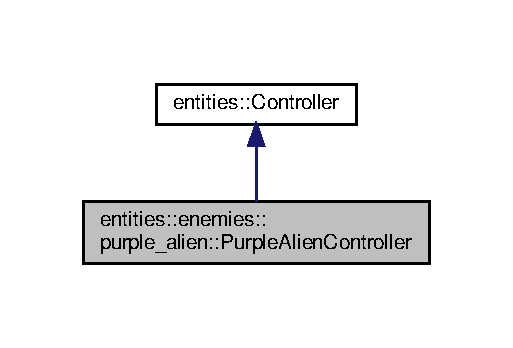
\includegraphics[width=246pt]{classentities_1_1enemies_1_1purple__alien_1_1PurpleAlienController__inherit__graph}
\end{center}
\end{figure}


Collaboration diagram for entities\+:\+:enemies\+:\+:purple\+\_\+alien\+:\+:Purple\+Alien\+Controller\+:\nopagebreak
\begin{figure}[H]
\begin{center}
\leavevmode
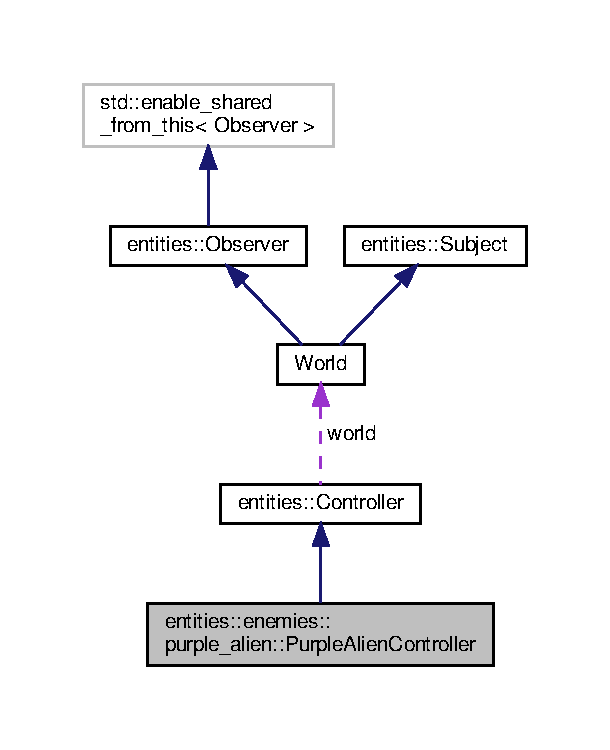
\includegraphics[width=293pt]{classentities_1_1enemies_1_1purple__alien_1_1PurpleAlienController__coll__graph}
\end{center}
\end{figure}
\subsection*{Public Member Functions}
\begin{DoxyCompactItemize}
\item 
\mbox{\Hypertarget{classentities_1_1enemies_1_1purple__alien_1_1PurpleAlienController_a4b88d417d2e14f4bc551be7b54aa31e1}\label{classentities_1_1enemies_1_1purple__alien_1_1PurpleAlienController_a4b88d417d2e14f4bc551be7b54aa31e1}} 
{\bfseries Purple\+Alien\+Controller} (const std\+::shared\+\_\+ptr$<$ \hyperlink{classentities_1_1Entity}{Entity} $>$ \&entity, const std\+::shared\+\_\+ptr$<$ \hyperlink{classentities_1_1View}{View} $>$ \&view, \hyperlink{classWorld}{World} \&world)
\item 
\mbox{\Hypertarget{classentities_1_1enemies_1_1purple__alien_1_1PurpleAlienController_a799cfca29a4cd55b64a7fa4fc5753d59}\label{classentities_1_1enemies_1_1purple__alien_1_1PurpleAlienController_a799cfca29a4cd55b64a7fa4fc5753d59}} 
bool {\bfseries handle\+Events} (const std\+::vector$<$ std\+::shared\+\_\+ptr$<$ \hyperlink{classentities_1_1Entity}{Entity} $>$$>$ \&entities) override
\end{DoxyCompactItemize}
\subsection*{Additional Inherited Members}


The documentation for this class was generated from the following files\+:\begin{DoxyCompactItemize}
\item 
/home/mano/\+Documents/univ/space\+\_\+invaders/src/entities/enemies/purple\+\_\+alien/\hyperlink{PurpleAlienController_8h}{Purple\+Alien\+Controller.\+h}\item 
/home/mano/\+Documents/univ/space\+\_\+invaders/src/entities/enemies/purple\+\_\+alien/\hyperlink{PurpleAlienController_8cpp}{Purple\+Alien\+Controller.\+cpp}\end{DoxyCompactItemize}

\hypertarget{classentities_1_1enemies_1_1purple__alien_1_1PurpleAlienView}{}\section{entities\+:\+:enemies\+:\+:purple\+\_\+alien\+:\+:Purple\+Alien\+View Class Reference}
\label{classentities_1_1enemies_1_1purple__alien_1_1PurpleAlienView}\index{entities\+::enemies\+::purple\+\_\+alien\+::\+Purple\+Alien\+View@{entities\+::enemies\+::purple\+\_\+alien\+::\+Purple\+Alien\+View}}


Inheritance diagram for entities\+:\+:enemies\+:\+:purple\+\_\+alien\+:\+:Purple\+Alien\+View\+:\nopagebreak
\begin{figure}[H]
\begin{center}
\leavevmode
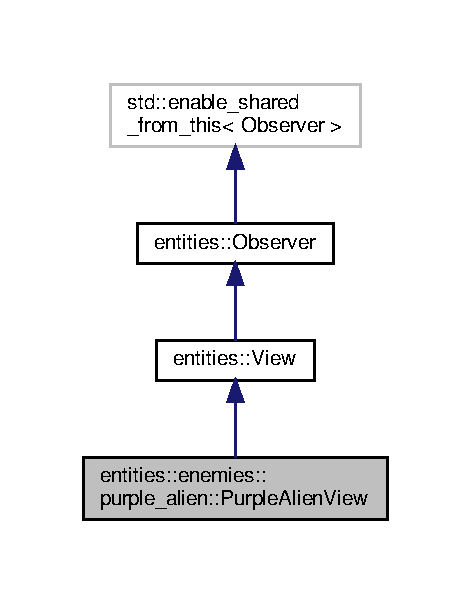
\includegraphics[width=226pt]{classentities_1_1enemies_1_1purple__alien_1_1PurpleAlienView__inherit__graph}
\end{center}
\end{figure}


Collaboration diagram for entities\+:\+:enemies\+:\+:purple\+\_\+alien\+:\+:Purple\+Alien\+View\+:\nopagebreak
\begin{figure}[H]
\begin{center}
\leavevmode
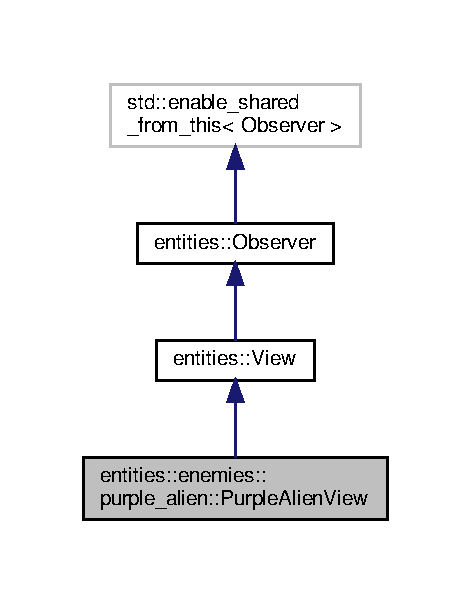
\includegraphics[width=226pt]{classentities_1_1enemies_1_1purple__alien_1_1PurpleAlienView__coll__graph}
\end{center}
\end{figure}
\subsection*{Public Member Functions}
\begin{DoxyCompactItemize}
\item 
\mbox{\Hypertarget{classentities_1_1enemies_1_1purple__alien_1_1PurpleAlienView_acb437c721aa9ee586ac8ce427a966cef}\label{classentities_1_1enemies_1_1purple__alien_1_1PurpleAlienView_acb437c721aa9ee586ac8ce427a966cef}} 
{\bfseries Purple\+Alien\+View} (const std\+::shared\+\_\+ptr$<$ \hyperlink{classentities_1_1enemies_1_1purple__alien_1_1PurpleAlien}{Purple\+Alien} $>$ \&alien)
\item 
\mbox{\Hypertarget{classentities_1_1enemies_1_1purple__alien_1_1PurpleAlienView_a1c0cd42fc59765b97724869601251590}\label{classentities_1_1enemies_1_1purple__alien_1_1PurpleAlienView_a1c0cd42fc59765b97724869601251590}} 
void {\bfseries on\+Notify} () override
\end{DoxyCompactItemize}
\subsection*{Additional Inherited Members}


The documentation for this class was generated from the following files\+:\begin{DoxyCompactItemize}
\item 
/home/mano/\+Documents/univ/space\+\_\+invaders/src/entities/enemies/purple\+\_\+alien/\hyperlink{PurpleAlienView_8h}{Purple\+Alien\+View.\+h}\item 
/home/mano/\+Documents/univ/space\+\_\+invaders/src/entities/enemies/purple\+\_\+alien/\hyperlink{PurpleAlienView_8cpp}{Purple\+Alien\+View.\+cpp}\end{DoxyCompactItemize}

\hypertarget{classobjects_1_1enemies_1_1red__alien_1_1RedAlien}{}\section{objects\+:\+:enemies\+:\+:red\+\_\+alien\+:\+:Red\+Alien Class Reference}
\label{classobjects_1_1enemies_1_1red__alien_1_1RedAlien}\index{objects\+::enemies\+::red\+\_\+alien\+::\+Red\+Alien@{objects\+::enemies\+::red\+\_\+alien\+::\+Red\+Alien}}


Inheritance diagram for objects\+:\+:enemies\+:\+:red\+\_\+alien\+:\+:Red\+Alien\+:\nopagebreak
\begin{figure}[H]
\begin{center}
\leavevmode
\includegraphics[width=181pt]{classobjects_1_1enemies_1_1red__alien_1_1RedAlien__inherit__graph}
\end{center}
\end{figure}


Collaboration diagram for objects\+:\+:enemies\+:\+:red\+\_\+alien\+:\+:Red\+Alien\+:\nopagebreak
\begin{figure}[H]
\begin{center}
\leavevmode
\includegraphics[width=181pt]{classobjects_1_1enemies_1_1red__alien_1_1RedAlien__coll__graph}
\end{center}
\end{figure}
\subsection*{Public Member Functions}
\begin{DoxyCompactItemize}
\item 
\mbox{\Hypertarget{classobjects_1_1enemies_1_1red__alien_1_1RedAlien_a481a0056973e547b92509fd4cced6282}\label{classobjects_1_1enemies_1_1red__alien_1_1RedAlien_a481a0056973e547b92509fd4cced6282}}
{\bfseries Red\+Alien} (float x, float y)
\item 
\mbox{\Hypertarget{classobjects_1_1enemies_1_1red__alien_1_1RedAlien_a29103fc5f6e44ea7b239b57fff8a1e59}\label{classobjects_1_1enemies_1_1red__alien_1_1RedAlien_a29103fc5f6e44ea7b239b57fff8a1e59}}
void {\bfseries update} () override
\end{DoxyCompactItemize}
\subsection*{Additional Inherited Members}


The documentation for this class was generated from the following files\+:\begin{DoxyCompactItemize}
\item 
/home/mano/\+Documents/univ/space\+\_\+invaders/src/objects/enemies/red\+\_\+alien/\hyperlink{RedAlien_8h}{Red\+Alien.\+h}\item
/home/mano/\+Documents/univ/space\+\_\+invaders/src/objects/enemies/red\+\_\+alien/\hyperlink{RedAlien_8cpp}{Red\+Alien.\+cpp}\end{DoxyCompactItemize}

\hypertarget{classentities_1_1enemies_1_1red__alien_1_1RedAlienController}{}\section{entities\+:\+:enemies\+:\+:red\+\_\+alien\+:\+:Red\+Alien\+Controller Class Reference}
\label{classentities_1_1enemies_1_1red__alien_1_1RedAlienController}\index{entities\+::enemies\+::red\+\_\+alien\+::\+Red\+Alien\+Controller@{entities\+::enemies\+::red\+\_\+alien\+::\+Red\+Alien\+Controller}}


Inheritance diagram for entities\+:\+:enemies\+:\+:red\+\_\+alien\+:\+:Red\+Alien\+Controller\+:\nopagebreak
\begin{figure}[H]
\begin{center}
\leavevmode
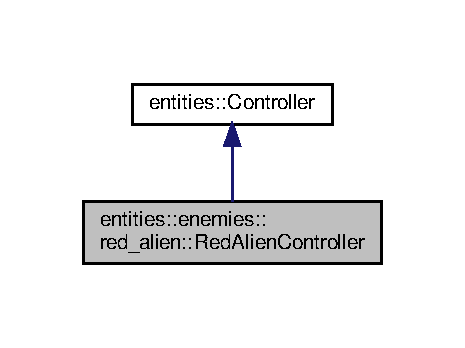
\includegraphics[width=223pt]{classentities_1_1enemies_1_1red__alien_1_1RedAlienController__inherit__graph}
\end{center}
\end{figure}


Collaboration diagram for entities\+:\+:enemies\+:\+:red\+\_\+alien\+:\+:Red\+Alien\+Controller\+:\nopagebreak
\begin{figure}[H]
\begin{center}
\leavevmode
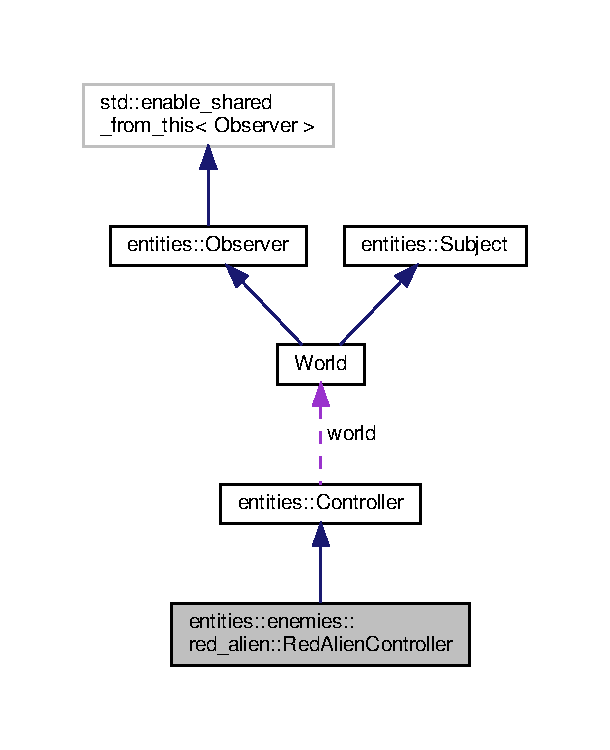
\includegraphics[width=293pt]{classentities_1_1enemies_1_1red__alien_1_1RedAlienController__coll__graph}
\end{center}
\end{figure}
\subsection*{Public Member Functions}
\begin{DoxyCompactItemize}
\item 
\mbox{\Hypertarget{classentities_1_1enemies_1_1red__alien_1_1RedAlienController_aebe17931bfbc588e09390846417684d5}\label{classentities_1_1enemies_1_1red__alien_1_1RedAlienController_aebe17931bfbc588e09390846417684d5}} 
{\bfseries Red\+Alien\+Controller} (const std\+::shared\+\_\+ptr$<$ \hyperlink{classentities_1_1Entity}{Entity} $>$ \&entity, const std\+::shared\+\_\+ptr$<$ \hyperlink{classentities_1_1View}{View} $>$ \&view, \hyperlink{classWorld}{World} \&world)
\item 
\mbox{\Hypertarget{classentities_1_1enemies_1_1red__alien_1_1RedAlienController_a60cd9e9d872c44c28827316255298e33}\label{classentities_1_1enemies_1_1red__alien_1_1RedAlienController_a60cd9e9d872c44c28827316255298e33}} 
bool {\bfseries handle\+Events} (const std\+::vector$<$ std\+::shared\+\_\+ptr$<$ \hyperlink{classentities_1_1Entity}{Entity} $>$$>$ \&entities) override
\end{DoxyCompactItemize}
\subsection*{Additional Inherited Members}


The documentation for this class was generated from the following files\+:\begin{DoxyCompactItemize}
\item 
/home/mano/\+Documents/univ/space\+\_\+invaders/src/entities/enemies/red\+\_\+alien/\hyperlink{RedAlienController_8h}{Red\+Alien\+Controller.\+h}\item 
/home/mano/\+Documents/univ/space\+\_\+invaders/src/entities/enemies/red\+\_\+alien/\hyperlink{RedAlienController_8cpp}{Red\+Alien\+Controller.\+cpp}\end{DoxyCompactItemize}

\hypertarget{classentities_1_1enemies_1_1red__alien_1_1RedAlienView}{}\section{entities\+:\+:enemies\+:\+:red\+\_\+alien\+:\+:Red\+Alien\+View Class Reference}
\label{classentities_1_1enemies_1_1red__alien_1_1RedAlienView}\index{entities\+::enemies\+::red\+\_\+alien\+::\+Red\+Alien\+View@{entities\+::enemies\+::red\+\_\+alien\+::\+Red\+Alien\+View}}


Inheritance diagram for entities\+:\+:enemies\+:\+:red\+\_\+alien\+:\+:Red\+Alien\+View\+:\nopagebreak
\begin{figure}[H]
\begin{center}
\leavevmode
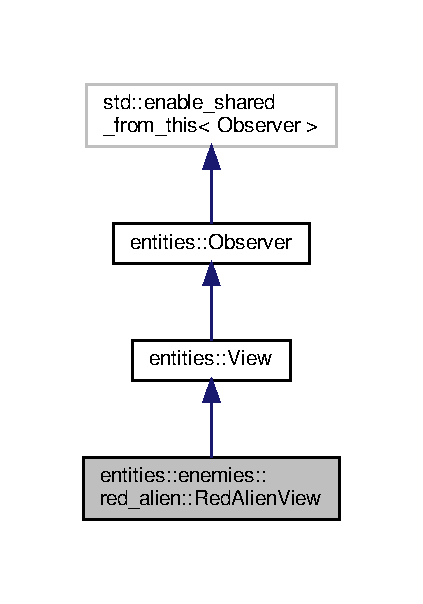
\includegraphics[width=203pt]{classentities_1_1enemies_1_1red__alien_1_1RedAlienView__inherit__graph}
\end{center}
\end{figure}


Collaboration diagram for entities\+:\+:enemies\+:\+:red\+\_\+alien\+:\+:Red\+Alien\+View\+:\nopagebreak
\begin{figure}[H]
\begin{center}
\leavevmode
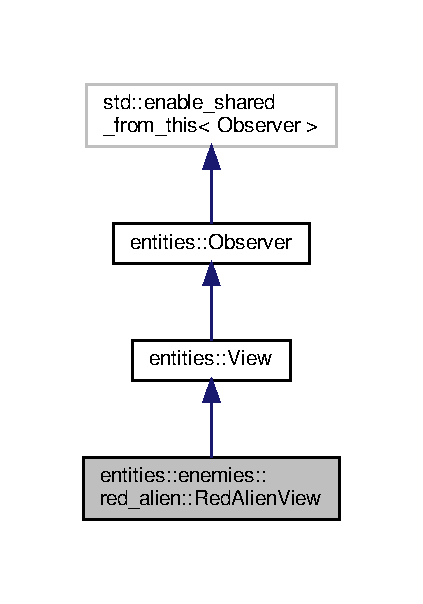
\includegraphics[width=203pt]{classentities_1_1enemies_1_1red__alien_1_1RedAlienView__coll__graph}
\end{center}
\end{figure}
\subsection*{Public Member Functions}
\begin{DoxyCompactItemize}
\item 
\mbox{\Hypertarget{classentities_1_1enemies_1_1red__alien_1_1RedAlienView_a291f78b84b87557b59bcf98d2cef95a6}\label{classentities_1_1enemies_1_1red__alien_1_1RedAlienView_a291f78b84b87557b59bcf98d2cef95a6}} 
{\bfseries Red\+Alien\+View} (const std\+::shared\+\_\+ptr$<$ \hyperlink{classentities_1_1enemies_1_1red__alien_1_1RedAlien}{Red\+Alien} $>$ \&enemy)
\item 
\mbox{\Hypertarget{classentities_1_1enemies_1_1red__alien_1_1RedAlienView_abddf987c883563442aa29a5bebfdfe9b}\label{classentities_1_1enemies_1_1red__alien_1_1RedAlienView_abddf987c883563442aa29a5bebfdfe9b}} 
void {\bfseries on\+Notify} () override
\end{DoxyCompactItemize}
\subsection*{Additional Inherited Members}


The documentation for this class was generated from the following files\+:\begin{DoxyCompactItemize}
\item 
/home/mano/\+Documents/univ/space\+\_\+invaders/src/entities/enemies/red\+\_\+alien/\hyperlink{RedAlienView_8h}{Red\+Alien\+View.\+h}\item 
/home/mano/\+Documents/univ/space\+\_\+invaders/src/entities/enemies/red\+\_\+alien/\hyperlink{RedAlienView_8cpp}{Red\+Alien\+View.\+cpp}\end{DoxyCompactItemize}

\hypertarget{classobjects_1_1shield_1_1Shield}{}\section{objects\+:\+:shield\+:\+:Shield Class Reference}
\label{classobjects_1_1shield_1_1Shield}\index{objects\+::shield\+::\+Shield@{objects\+::shield\+::\+Shield}}


Inheritance diagram for objects\+:\+:shield\+:\+:Shield\+:\nopagebreak
\begin{figure}[H]
\begin{center}
\leavevmode
\includegraphics[width=193pt]{classobjects_1_1shield_1_1Shield__inherit__graph}
\end{center}
\end{figure}


Collaboration diagram for objects\+:\+:shield\+:\+:Shield\+:\nopagebreak
\begin{figure}[H]
\begin{center}
\leavevmode
\includegraphics[width=193pt]{classobjects_1_1shield_1_1Shield__coll__graph}
\end{center}
\end{figure}
\subsection*{Public Member Functions}
\begin{DoxyCompactItemize}
\item 
\mbox{\Hypertarget{classobjects_1_1shield_1_1Shield_a2fcfb95c4bca077c3d284538bbdf4559}\label{classobjects_1_1shield_1_1Shield_a2fcfb95c4bca077c3d284538bbdf4559}}
{\bfseries Shield} (float x, float y)
\item 
\mbox{\Hypertarget{classobjects_1_1shield_1_1Shield_a78b754cf93dea3796d144d9eca664d69}\label{classobjects_1_1shield_1_1Shield_a78b754cf93dea3796d144d9eca664d69}}
void {\bfseries update} () override
\end{DoxyCompactItemize}
\subsection*{Additional Inherited Members}


The documentation for this class was generated from the following files\+:\begin{DoxyCompactItemize}
\item 
/home/mano/\+Documents/univ/space\+\_\+invaders/src/objects/shield/\hyperlink{Shield_8h}{Shield.\+h}\item
/home/mano/\+Documents/univ/space\+\_\+invaders/src/objects/shield/\hyperlink{Shield_8cpp}{Shield.\+cpp}\end{DoxyCompactItemize}

\hypertarget{classobjects_1_1shield_1_1ShieldController}{}\section{objects\+:\+:shield\+:\+:Shield\+Controller Class Reference}
\label{classobjects_1_1shield_1_1ShieldController}\index{objects\+::shield\+::\+Shield\+Controller@{objects\+::shield\+::\+Shield\+Controller}}


Inheritance diagram for objects\+:\+:shield\+:\+:Shield\+Controller\+:\nopagebreak
\begin{figure}[H]
\begin{center}
\leavevmode
\includegraphics[width=193pt]{classobjects_1_1shield_1_1ShieldController__inherit__graph}
\end{center}
\end{figure}


Collaboration diagram for objects\+:\+:shield\+:\+:Shield\+Controller\+:\nopagebreak
\begin{figure}[H]
\begin{center}
\leavevmode
\includegraphics[width=293pt]{classobjects_1_1shield_1_1ShieldController__coll__graph}
\end{center}
\end{figure}
\subsection*{Public Member Functions}
\begin{DoxyCompactItemize}
\item 
\mbox{\Hypertarget{classobjects_1_1shield_1_1ShieldController_a91b1b04f46545a50201c14bd1fbda530}\label{classobjects_1_1shield_1_1ShieldController_a91b1b04f46545a50201c14bd1fbda530}}
{\bfseries Shield\+Controller} (const std\+::shared\+\_\+ptr$<$ \hyperlink{classobjects_1_1Entity}{Entity} $>$ \&entity, const std\+::shared\+\_\+ptr$<$ \hyperlink{classobjects_1_1View}{View} $>$ \&view, \hyperlink{classWorld}{World} \&world)
\item 
\mbox{\Hypertarget{classobjects_1_1shield_1_1ShieldController_a0c1bacca0231a39a1614147f65437987}\label{classobjects_1_1shield_1_1ShieldController_a0c1bacca0231a39a1614147f65437987}}
bool {\bfseries handle\+Events} (const std\+::vector$<$ std\+::shared\+\_\+ptr$<$ \hyperlink{classobjects_1_1Entity}{Entity} $>$$>$ \&objects) override
\end{DoxyCompactItemize}
\subsection*{Additional Inherited Members}


The documentation for this class was generated from the following files\+:\begin{DoxyCompactItemize}
\item 
/home/mano/\+Documents/univ/space\+\_\+invaders/src/objects/shield/\hyperlink{ShieldController_8h}{Shield\+Controller.\+h}\item
/home/mano/\+Documents/univ/space\+\_\+invaders/src/objects/shield/\hyperlink{ShieldController_8cpp}{Shield\+Controller.\+cpp}\end{DoxyCompactItemize}

\hypertarget{classobjects_1_1shield_1_1ShieldView}{}\section{objects\+:\+:shield\+:\+:Shield\+View Class Reference}
\label{classobjects_1_1shield_1_1ShieldView}\index{objects\+::shield\+::\+Shield\+View@{objects\+::shield\+::\+Shield\+View}}


Inheritance diagram for objects\+:\+:shield\+:\+:Shield\+View\+:\nopagebreak
\begin{figure}[H]
\begin{center}
\leavevmode
\includegraphics[width=214pt]{classobjects_1_1shield_1_1ShieldView__inherit__graph}
\end{center}
\end{figure}


Collaboration diagram for objects\+:\+:shield\+:\+:Shield\+View\+:\nopagebreak
\begin{figure}[H]
\begin{center}
\leavevmode
\includegraphics[width=214pt]{classobjects_1_1shield_1_1ShieldView__coll__graph}
\end{center}
\end{figure}
\subsection*{Public Member Functions}
\begin{DoxyCompactItemize}
\item 
\mbox{\Hypertarget{classobjects_1_1shield_1_1ShieldView_ac2f9dbbdc6efd8a3453576c83d62a8fe}\label{classobjects_1_1shield_1_1ShieldView_ac2f9dbbdc6efd8a3453576c83d62a8fe}}
{\bfseries Shield\+View} (const std\+::shared\+\_\+ptr$<$ \hyperlink{classobjects_1_1Entity}{Entity} $>$ \&entity)
\item 
\mbox{\Hypertarget{classobjects_1_1shield_1_1ShieldView_ab1646d34b45e9007c12fbf03b81222f2}\label{classobjects_1_1shield_1_1ShieldView_ab1646d34b45e9007c12fbf03b81222f2}}
void {\bfseries on\+Notify} () override
\end{DoxyCompactItemize}
\subsection*{Additional Inherited Members}


The documentation for this class was generated from the following files\+:\begin{DoxyCompactItemize}
\item 
/home/mano/\+Documents/univ/space\+\_\+invaders/src/objects/shield/\hyperlink{ShieldView_8h}{Shield\+View.\+h}\item
/home/mano/\+Documents/univ/space\+\_\+invaders/src/objects/shield/\hyperlink{ShieldView_8cpp}{Shield\+View.\+cpp}\end{DoxyCompactItemize}

\input{classutil_1_1SpaceSettings}
\hypertarget{classentities_1_1projectiles_1_1standard__enemy_1_1StandardEnemyProjectile}{}\section{entities\+:\+:projectiles\+:\+:standard\+\_\+enemy\+:\+:Standard\+Enemy\+Projectile Class Reference}
\label{classentities_1_1projectiles_1_1standard__enemy_1_1StandardEnemyProjectile}\index{entities\+::projectiles\+::standard\+\_\+enemy\+::\+Standard\+Enemy\+Projectile@{entities\+::projectiles\+::standard\+\_\+enemy\+::\+Standard\+Enemy\+Projectile}}


Inheritance diagram for entities\+:\+:projectiles\+:\+:standard\+\_\+enemy\+:\+:Standard\+Enemy\+Projectile\+:\nopagebreak
\begin{figure}[H]
\begin{center}
\leavevmode
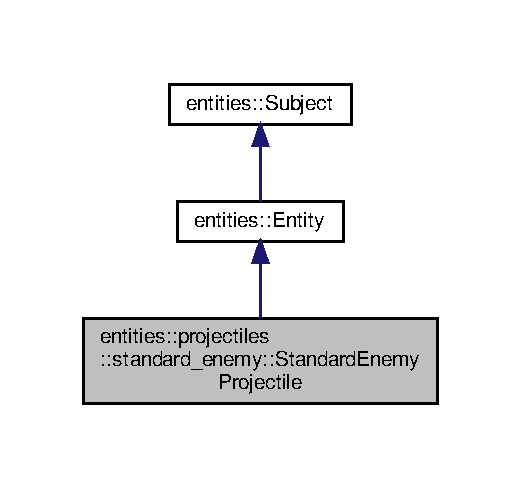
\includegraphics[width=250pt]{classentities_1_1projectiles_1_1standard__enemy_1_1StandardEnemyProjectile__inherit__graph}
\end{center}
\end{figure}


Collaboration diagram for entities\+:\+:projectiles\+:\+:standard\+\_\+enemy\+:\+:Standard\+Enemy\+Projectile\+:\nopagebreak
\begin{figure}[H]
\begin{center}
\leavevmode
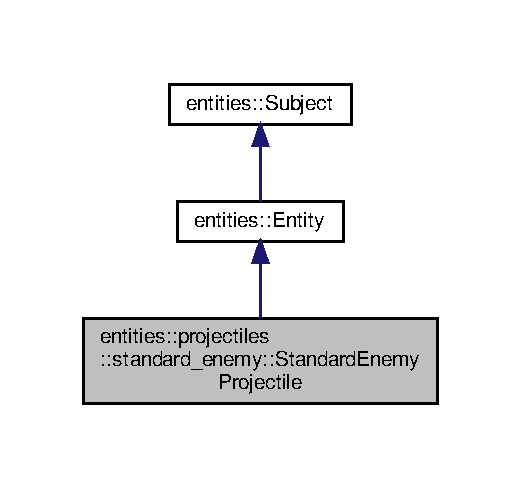
\includegraphics[width=250pt]{classentities_1_1projectiles_1_1standard__enemy_1_1StandardEnemyProjectile__coll__graph}
\end{center}
\end{figure}
\subsection*{Public Member Functions}
\begin{DoxyCompactItemize}
\item 
\mbox{\Hypertarget{classentities_1_1projectiles_1_1standard__enemy_1_1StandardEnemyProjectile_abc3abd0c8b7d2ff776bf55ab04be67c3}\label{classentities_1_1projectiles_1_1standard__enemy_1_1StandardEnemyProjectile_abc3abd0c8b7d2ff776bf55ab04be67c3}} 
{\bfseries Standard\+Enemy\+Projectile} (float x, float y)
\item 
\mbox{\Hypertarget{classentities_1_1projectiles_1_1standard__enemy_1_1StandardEnemyProjectile_a8a5890e9986800df9870c26c83950743}\label{classentities_1_1projectiles_1_1standard__enemy_1_1StandardEnemyProjectile_a8a5890e9986800df9870c26c83950743}} 
void {\bfseries move} ()
\item 
\mbox{\Hypertarget{classentities_1_1projectiles_1_1standard__enemy_1_1StandardEnemyProjectile_a9c48f6f68fddcd9d9e7c5a610eba2af8}\label{classentities_1_1projectiles_1_1standard__enemy_1_1StandardEnemyProjectile_a9c48f6f68fddcd9d9e7c5a610eba2af8}} 
void {\bfseries update} () override
\end{DoxyCompactItemize}
\subsection*{Additional Inherited Members}


The documentation for this class was generated from the following files\+:\begin{DoxyCompactItemize}
\item 
/home/mano/\+Documents/univ/space\+\_\+invaders/src/entities/projectiles/standard\+\_\+enemy/\hyperlink{StandardEnemyProjectile_8h}{Standard\+Enemy\+Projectile.\+h}\item 
/home/mano/\+Documents/univ/space\+\_\+invaders/src/entities/projectiles/standard\+\_\+enemy/\hyperlink{StandardEnemyProjectile_8cpp}{Standard\+Enemy\+Projectile.\+cpp}\end{DoxyCompactItemize}

\hypertarget{classobjects_1_1projectiles_1_1standard__enemy_1_1StandardEnemyProjectileController}{}\section{objects\+:\+:projectiles\+:\+:standard\+\_\+enemy\+:\+:Standard\+Enemy\+Projectile\+Controller Class Reference}
\label{classobjects_1_1projectiles_1_1standard__enemy_1_1StandardEnemyProjectileController}\index{objects\+::projectiles\+::standard\+\_\+enemy\+::\+Standard\+Enemy\+Projectile\+Controller@{objects\+::projectiles\+::standard\+\_\+enemy\+::\+Standard\+Enemy\+Projectile\+Controller}}


Inheritance diagram for objects\+:\+:projectiles\+:\+:standard\+\_\+enemy\+:\+:Standard\+Enemy\+Projectile\+Controller\+:\nopagebreak
\begin{figure}[H]
\begin{center}
\leavevmode
\includegraphics[width=250pt]{classobjects_1_1projectiles_1_1standard__enemy_1_1StandardEnemyProjectileController__inherit__graph}
\end{center}
\end{figure}


Collaboration diagram for objects\+:\+:projectiles\+:\+:standard\+\_\+enemy\+:\+:Standard\+Enemy\+Projectile\+Controller\+:\nopagebreak
\begin{figure}[H]
\begin{center}
\leavevmode
\includegraphics[width=293pt]{classobjects_1_1projectiles_1_1standard__enemy_1_1StandardEnemyProjectileController__coll__graph}
\end{center}
\end{figure}
\subsection*{Public Member Functions}
\begin{DoxyCompactItemize}
\item 
\mbox{\Hypertarget{classobjects_1_1projectiles_1_1standard__enemy_1_1StandardEnemyProjectileController_a606a41a83cf137d079d02a1082b3d4e7}\label{classobjects_1_1projectiles_1_1standard__enemy_1_1StandardEnemyProjectileController_a606a41a83cf137d079d02a1082b3d4e7}}
{\bfseries Standard\+Enemy\+Projectile\+Controller} (const std\+::shared\+\_\+ptr$<$ \hyperlink{classobjects_1_1Entity}{Entity} $>$ \&entity, const std\+::shared\+\_\+ptr$<$ \hyperlink{classobjects_1_1View}{View} $>$ \&view, \hyperlink{classWorld}{World} \&world)
\item 
\mbox{\Hypertarget{classobjects_1_1projectiles_1_1standard__enemy_1_1StandardEnemyProjectileController_ab462caef5dfc423f8f6fcdb195d59676}\label{classobjects_1_1projectiles_1_1standard__enemy_1_1StandardEnemyProjectileController_ab462caef5dfc423f8f6fcdb195d59676}}
bool {\bfseries handle\+Events} (const std\+::vector$<$ std\+::shared\+\_\+ptr$<$ \hyperlink{classobjects_1_1Entity}{Entity} $>$$>$ \&objects) override
\end{DoxyCompactItemize}
\subsection*{Additional Inherited Members}


The documentation for this class was generated from the following files\+:\begin{DoxyCompactItemize}
\item 
/home/mano/\+Documents/univ/space\+\_\+invaders/src/objects/projectiles/standard\+\_\+enemy/\hyperlink{StandardEnemyProjectileController_8h}{Standard\+Enemy\+Projectile\+Controller.\+h}\item
/home/mano/\+Documents/univ/space\+\_\+invaders/src/objects/projectiles/standard\+\_\+enemy/\hyperlink{StandardEnemyProjectileController_8cpp}{Standard\+Enemy\+Projectile\+Controller.\+cpp}\end{DoxyCompactItemize}

\hypertarget{classobjects_1_1projectiles_1_1standard__enemy_1_1StandardEnemyProjectileView}{}\section{objects\+:\+:projectiles\+:\+:standard\+\_\+enemy\+:\+:Standard\+Enemy\+Projectile\+View Class Reference}
\label{classobjects_1_1projectiles_1_1standard__enemy_1_1StandardEnemyProjectileView}\index{objects\+::projectiles\+::standard\+\_\+enemy\+::\+Standard\+Enemy\+Projectile\+View@{objects\+::projectiles\+::standard\+\_\+enemy\+::\+Standard\+Enemy\+Projectile\+View}}


Inheritance diagram for objects\+:\+:projectiles\+:\+:standard\+\_\+enemy\+:\+:Standard\+Enemy\+Projectile\+View\+:\nopagebreak
\begin{figure}[H]
\begin{center}
\leavevmode
\includegraphics[width=250pt]{classobjects_1_1projectiles_1_1standard__enemy_1_1StandardEnemyProjectileView__inherit__graph}
\end{center}
\end{figure}


Collaboration diagram for objects\+:\+:projectiles\+:\+:standard\+\_\+enemy\+:\+:Standard\+Enemy\+Projectile\+View\+:\nopagebreak
\begin{figure}[H]
\begin{center}
\leavevmode
\includegraphics[width=250pt]{classobjects_1_1projectiles_1_1standard__enemy_1_1StandardEnemyProjectileView__coll__graph}
\end{center}
\end{figure}
\subsection*{Public Member Functions}
\begin{DoxyCompactItemize}
\item 
\mbox{\Hypertarget{classobjects_1_1projectiles_1_1standard__enemy_1_1StandardEnemyProjectileView_a427269c9aa0e8b59e424dda56e8bb3cd}\label{classobjects_1_1projectiles_1_1standard__enemy_1_1StandardEnemyProjectileView_a427269c9aa0e8b59e424dda56e8bb3cd}}
{\bfseries Standard\+Enemy\+Projectile\+View} (const std\+::shared\+\_\+ptr$<$ \hyperlink{classobjects_1_1projectiles_1_1standard__enemy_1_1StandardEnemyProjectile}{Standard\+Enemy\+Projectile} $>$ \&projectile)
\item 
\mbox{\Hypertarget{classobjects_1_1projectiles_1_1standard__enemy_1_1StandardEnemyProjectileView_a25fd3839b1dc9964fd256650a82c8237}\label{classobjects_1_1projectiles_1_1standard__enemy_1_1StandardEnemyProjectileView_a25fd3839b1dc9964fd256650a82c8237}}
void {\bfseries on\+Notify} () override
\end{DoxyCompactItemize}
\subsection*{Additional Inherited Members}


The documentation for this class was generated from the following files\+:\begin{DoxyCompactItemize}
\item 
/home/mano/\+Documents/univ/space\+\_\+invaders/src/objects/projectiles/standard\+\_\+enemy/\hyperlink{StandardEnemyProjectileView_8h}{Standard\+Enemy\+Projectile\+View.\+h}\item
/home/mano/\+Documents/univ/space\+\_\+invaders/src/objects/projectiles/standard\+\_\+enemy/\hyperlink{StandardEnemyProjectileView_8cpp}{Standard\+Enemy\+Projectile\+View.\+cpp}\end{DoxyCompactItemize}

\hypertarget{classobjects_1_1projectiles_1_1standard_1_1StandardProjectile}{}\section{objects\+:\+:projectiles\+:\+:standard\+:\+:Standard\+Projectile Class Reference}
\label{classobjects_1_1projectiles_1_1standard_1_1StandardProjectile}\index{objects\+::projectiles\+::standard\+::\+Standard\+Projectile@{objects\+::projectiles\+::standard\+::\+Standard\+Projectile}}


Inheritance diagram for objects\+:\+:projectiles\+:\+:standard\+:\+:Standard\+Projectile\+:\nopagebreak
\begin{figure}[H]
\begin{center}
\leavevmode
\includegraphics[width=226pt]{classobjects_1_1projectiles_1_1standard_1_1StandardProjectile__inherit__graph}
\end{center}
\end{figure}


Collaboration diagram for objects\+:\+:projectiles\+:\+:standard\+:\+:Standard\+Projectile\+:\nopagebreak
\begin{figure}[H]
\begin{center}
\leavevmode
\includegraphics[width=226pt]{classobjects_1_1projectiles_1_1standard_1_1StandardProjectile__coll__graph}
\end{center}
\end{figure}
\subsection*{Public Member Functions}
\begin{DoxyCompactItemize}
\item 
\mbox{\Hypertarget{classobjects_1_1projectiles_1_1standard_1_1StandardProjectile_a36a576f2cbb69f86b100a089591f190c}\label{classobjects_1_1projectiles_1_1standard_1_1StandardProjectile_a36a576f2cbb69f86b100a089591f190c}}
{\bfseries Standard\+Projectile} (float x, float y)
\item 
\mbox{\Hypertarget{classobjects_1_1projectiles_1_1standard_1_1StandardProjectile_a02b8c02279340f88b3143eb75d4257a8}\label{classobjects_1_1projectiles_1_1standard_1_1StandardProjectile_a02b8c02279340f88b3143eb75d4257a8}}
void {\bfseries move} ()
\item 
\mbox{\Hypertarget{classobjects_1_1projectiles_1_1standard_1_1StandardProjectile_a51122df8dc5e0fb55317e18f45c5f24e}\label{classobjects_1_1projectiles_1_1standard_1_1StandardProjectile_a51122df8dc5e0fb55317e18f45c5f24e}}
void {\bfseries update} () override
\end{DoxyCompactItemize}
\subsection*{Additional Inherited Members}


The documentation for this class was generated from the following files\+:\begin{DoxyCompactItemize}
\item 
/home/mano/\+Documents/univ/space\+\_\+invaders/src/objects/projectiles/standard/\hyperlink{StandardProjectile_8h}{Standard\+Projectile.\+h}\item
/home/mano/\+Documents/univ/space\+\_\+invaders/src/objects/projectiles/standard/\hyperlink{StandardProjectile_8cpp}{Standard\+Projectile.\+cpp}\end{DoxyCompactItemize}

\hypertarget{classentities_1_1projectiles_1_1standard_1_1StandardProjectileController}{}\section{entities\+:\+:projectiles\+:\+:standard\+:\+:Standard\+Projectile\+Controller Class Reference}
\label{classentities_1_1projectiles_1_1standard_1_1StandardProjectileController}\index{entities\+::projectiles\+::standard\+::\+Standard\+Projectile\+Controller@{entities\+::projectiles\+::standard\+::\+Standard\+Projectile\+Controller}}


Inheritance diagram for entities\+:\+:projectiles\+:\+:standard\+:\+:Standard\+Projectile\+Controller\+:\nopagebreak
\begin{figure}[H]
\begin{center}
\leavevmode
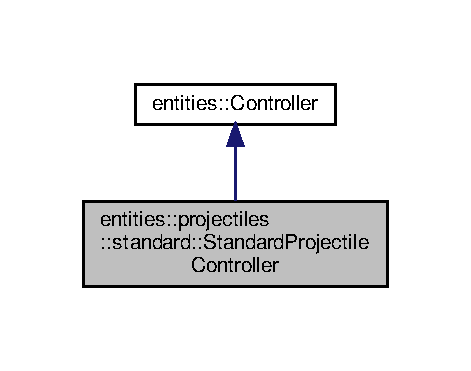
\includegraphics[width=226pt]{classentities_1_1projectiles_1_1standard_1_1StandardProjectileController__inherit__graph}
\end{center}
\end{figure}


Collaboration diagram for entities\+:\+:projectiles\+:\+:standard\+:\+:Standard\+Projectile\+Controller\+:\nopagebreak
\begin{figure}[H]
\begin{center}
\leavevmode
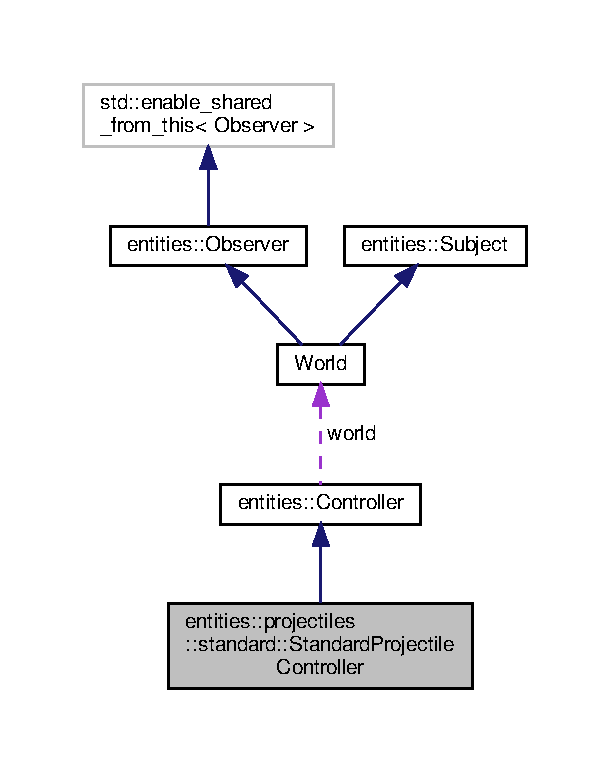
\includegraphics[width=293pt]{classentities_1_1projectiles_1_1standard_1_1StandardProjectileController__coll__graph}
\end{center}
\end{figure}
\subsection*{Public Member Functions}
\begin{DoxyCompactItemize}
\item 
\mbox{\Hypertarget{classentities_1_1projectiles_1_1standard_1_1StandardProjectileController_a9d31e5fdb4680c3ce373bfb494a5920e}\label{classentities_1_1projectiles_1_1standard_1_1StandardProjectileController_a9d31e5fdb4680c3ce373bfb494a5920e}} 
{\bfseries Standard\+Projectile\+Controller} (const std\+::shared\+\_\+ptr$<$ \hyperlink{classentities_1_1Entity}{Entity} $>$ \&entity, const std\+::shared\+\_\+ptr$<$ \hyperlink{classentities_1_1View}{View} $>$ \&view, \hyperlink{classWorld}{World} \&world)
\item 
\mbox{\Hypertarget{classentities_1_1projectiles_1_1standard_1_1StandardProjectileController_ad591fceeeebeb569a4d5a1915cadaa6b}\label{classentities_1_1projectiles_1_1standard_1_1StandardProjectileController_ad591fceeeebeb569a4d5a1915cadaa6b}} 
bool {\bfseries handle\+Events} (const std\+::vector$<$ std\+::shared\+\_\+ptr$<$ \hyperlink{classentities_1_1Entity}{Entity} $>$$>$ \&entities) override
\end{DoxyCompactItemize}
\subsection*{Additional Inherited Members}


The documentation for this class was generated from the following files\+:\begin{DoxyCompactItemize}
\item 
/home/mano/\+Documents/univ/space\+\_\+invaders/src/entities/projectiles/standard/\hyperlink{StandardProjectileController_8h}{Standard\+Projectile\+Controller.\+h}\item 
/home/mano/\+Documents/univ/space\+\_\+invaders/src/entities/projectiles/standard/\hyperlink{StandardProjectileController_8cpp}{Standard\+Projectile\+Controller.\+cpp}\end{DoxyCompactItemize}

\hypertarget{classobjects_1_1projectiles_1_1standard_1_1StandardProjectileView}{}\section{objects\+:\+:projectiles\+:\+:standard\+:\+:Standard\+Projectile\+View Class Reference}
\label{classobjects_1_1projectiles_1_1standard_1_1StandardProjectileView}\index{objects\+::projectiles\+::standard\+::\+Standard\+Projectile\+View@{objects\+::projectiles\+::standard\+::\+Standard\+Projectile\+View}}


Inheritance diagram for objects\+:\+:projectiles\+:\+:standard\+:\+:Standard\+Projectile\+View\+:\nopagebreak
\begin{figure}[H]
\begin{center}
\leavevmode
\includegraphics[width=247pt]{classobjects_1_1projectiles_1_1standard_1_1StandardProjectileView__inherit__graph}
\end{center}
\end{figure}


Collaboration diagram for objects\+:\+:projectiles\+:\+:standard\+:\+:Standard\+Projectile\+View\+:\nopagebreak
\begin{figure}[H]
\begin{center}
\leavevmode
\includegraphics[width=247pt]{classobjects_1_1projectiles_1_1standard_1_1StandardProjectileView__coll__graph}
\end{center}
\end{figure}
\subsection*{Public Member Functions}
\begin{DoxyCompactItemize}
\item 
\mbox{\Hypertarget{classobjects_1_1projectiles_1_1standard_1_1StandardProjectileView_a93bc0e6f5a422406185e4d99b2e0f83e}\label{classobjects_1_1projectiles_1_1standard_1_1StandardProjectileView_a93bc0e6f5a422406185e4d99b2e0f83e}}
{\bfseries Standard\+Projectile\+View} (const std\+::shared\+\_\+ptr$<$ \hyperlink{classobjects_1_1projectiles_1_1standard_1_1StandardProjectile}{Standard\+Projectile} $>$ \&projectile)
\item 
\mbox{\Hypertarget{classobjects_1_1projectiles_1_1standard_1_1StandardProjectileView_a8afdc8dc0deace3a76b1b43ca0e1b251}\label{classobjects_1_1projectiles_1_1standard_1_1StandardProjectileView_a8afdc8dc0deace3a76b1b43ca0e1b251}}
void {\bfseries on\+Notify} () override
\end{DoxyCompactItemize}
\subsection*{Additional Inherited Members}


The documentation for this class was generated from the following files\+:\begin{DoxyCompactItemize}
\item 
/home/mano/\+Documents/univ/space\+\_\+invaders/src/objects/projectiles/standard/\hyperlink{StandardProjectileView_8h}{Standard\+Projectile\+View.\+h}\item
/home/mano/\+Documents/univ/space\+\_\+invaders/src/objects/projectiles/standard/\hyperlink{StandardProjectileView_8cpp}{Standard\+Projectile\+View.\+cpp}\end{DoxyCompactItemize}

\input{classutil_1_1Stopwatch}
\hypertarget{classentities_1_1Subject}{}\section{entities\+:\+:Subject Class Reference}
\label{classentities_1_1Subject}\index{entities\+::\+Subject@{entities\+::\+Subject}}


Inheritance diagram for entities\+:\+:Subject\+:\nopagebreak
\begin{figure}[H]
\begin{center}
\leavevmode
\includegraphics[width=350pt]{classentities_1_1Subject__inherit__graph}
\end{center}
\end{figure}
\subsection*{Public Member Functions}
\begin{DoxyCompactItemize}
\item 
\mbox{\Hypertarget{classentities_1_1Subject_a17c678c4c3c50a76fd972952a7e7ca75}\label{classentities_1_1Subject_a17c678c4c3c50a76fd972952a7e7ca75}} 
void {\bfseries attach} (std\+::weak\+\_\+ptr$<$ \hyperlink{classentities_1_1Observer}{Observer} $>$ observer)
\end{DoxyCompactItemize}
\subsection*{Protected Member Functions}
\begin{DoxyCompactItemize}
\item 
\mbox{\Hypertarget{classentities_1_1Subject_a2562dcbae6bbb26ce21cec268fe5ed41}\label{classentities_1_1Subject_a2562dcbae6bbb26ce21cec268fe5ed41}} 
void {\bfseries on\+Notify\+Observers} () const
\end{DoxyCompactItemize}
\subsection*{Protected Attributes}
\begin{DoxyCompactItemize}
\item 
\mbox{\Hypertarget{classentities_1_1Subject_a3764a6f9d547038483f139cc72061c44}\label{classentities_1_1Subject_a3764a6f9d547038483f139cc72061c44}} 
std\+::vector$<$ std\+::weak\+\_\+ptr$<$ \hyperlink{classentities_1_1Observer}{Observer} $>$ $>$ {\bfseries observers}
\end{DoxyCompactItemize}


The documentation for this class was generated from the following file\+:\begin{DoxyCompactItemize}
\item 
/home/mano/\+Documents/univ/space\+\_\+invaders/src/entities/abstract\+\_\+classes/\hyperlink{Subject_8h}{Subject.\+h}\end{DoxyCompactItemize}

\input{classutil_1_1Transformation}
\hypertarget{classentities_1_1View}{}\section{entities\+:\+:View Class Reference}
\label{classentities_1_1View}\index{entities\+::\+View@{entities\+::\+View}}


Inheritance diagram for entities\+:\+:View\+:\nopagebreak
\begin{figure}[H]
\begin{center}
\leavevmode
\includegraphics[width=350pt]{classentities_1_1View__inherit__graph}
\end{center}
\end{figure}


Collaboration diagram for entities\+:\+:View\+:\nopagebreak
\begin{figure}[H]
\begin{center}
\leavevmode
\includegraphics[width=200pt]{classentities_1_1View__coll__graph}
\end{center}
\end{figure}
\subsection*{Public Member Functions}
\begin{DoxyCompactItemize}
\item 
\mbox{\Hypertarget{classentities_1_1View_ad552142da711120077dd6bb27c8f7b5f}\label{classentities_1_1View_ad552142da711120077dd6bb27c8f7b5f}} 
virtual void {\bfseries draw} (sf\+::\+Render\+Window \&window) const
\item 
\mbox{\Hypertarget{classentities_1_1View_a3aff15a86a88ee075251cd69d6d23926}\label{classentities_1_1View_a3aff15a86a88ee075251cd69d6d23926}} 
void {\bfseries init} ()
\end{DoxyCompactItemize}
\subsection*{Protected Member Functions}
\begin{DoxyCompactItemize}
\item 
\mbox{\Hypertarget{classentities_1_1View_adc22291b6660cef23f325773b21cc476}\label{classentities_1_1View_adc22291b6660cef23f325773b21cc476}} 
{\bfseries View} (const std\+::string \&image, std\+::shared\+\_\+ptr$<$ \hyperlink{classentities_1_1Entity}{Entity} $>$ shared\+Ptr)
\end{DoxyCompactItemize}
\subsection*{Protected Attributes}
\begin{DoxyCompactItemize}
\item 
\mbox{\Hypertarget{classentities_1_1View_aacd0b5eb20efc07425ba1fdde39aaebe}\label{classentities_1_1View_aacd0b5eb20efc07425ba1fdde39aaebe}} 
std\+::shared\+\_\+ptr$<$ \hyperlink{classentities_1_1Entity}{Entity} $>$ {\bfseries entity}
\item 
\mbox{\Hypertarget{classentities_1_1View_a8d21dfa5a6479b509e0c7806d2637d2a}\label{classentities_1_1View_a8d21dfa5a6479b509e0c7806d2637d2a}} 
std\+::unique\+\_\+ptr$<$ sf\+::\+Sprite $>$ {\bfseries sprite}
\item 
\mbox{\Hypertarget{classentities_1_1View_a9858db6cad1df3649e96a3aaa9edea7e}\label{classentities_1_1View_a9858db6cad1df3649e96a3aaa9edea7e}} 
std\+::unique\+\_\+ptr$<$ sf\+::\+Texture $>$ {\bfseries texture}
\item 
\mbox{\Hypertarget{classentities_1_1View_ae2ebde4944e5808450d560508bf722a6}\label{classentities_1_1View_ae2ebde4944e5808450d560508bf722a6}} 
bool {\bfseries initialized} = false
\end{DoxyCompactItemize}


The documentation for this class was generated from the following files\+:\begin{DoxyCompactItemize}
\item 
/home/mano/\+Documents/univ/space\+\_\+invaders/src/entities/abstract\+\_\+classes/\hyperlink{View_8h}{View.\+h}\item 
/home/mano/\+Documents/univ/space\+\_\+invaders/src/entities/abstract\+\_\+classes/\hyperlink{View_8cpp}{View.\+cpp}\end{DoxyCompactItemize}

\hypertarget{classWorld}{}\section{World Class Reference}
\label{classWorld}\index{World@{World}}


Inheritance diagram for World\+:
\nopagebreak
\begin{figure}[H]
\begin{center}
\leavevmode
\includegraphics[width=200pt]{classWorld__inherit__graph}
\end{center}
\end{figure}


Collaboration diagram for World\+:
\nopagebreak
\begin{figure}[H]
\begin{center}
\leavevmode
\includegraphics[width=200pt]{classWorld__coll__graph}
\end{center}
\end{figure}
\subsection*{Public Member Functions}
\begin{DoxyCompactItemize}
\item 
\hyperlink{classWorld_a96ca734b18df2cf85e666fc6d358e12c}{World} (std\+::shared\+\_\+ptr$<$ sf\+::\+Render\+Window $>$ window\+Ptr)
\item 
void \hyperlink{classWorld_a6a08c827c3a0def12b7700211353735f}{load\+Level} (const std\+::string \&filename)
\item 
void \hyperlink{classWorld_a91c2d7b127190f17a6cd85743245fb5b}{on\+Notify} () override
\item 
void \hyperlink{classWorld_ad37fe32cce284282361b9e7397b27a23}{handle\+Events} ()
\item 
void \hyperlink{classWorld_a5cc73b1aa54db5da01e4004acd4fd8bb}{update\+Entities} ()
\item 
void \hyperlink{classWorld_a8e8ad60668f8fe975f03bcb612264bc4}{draw\+Views} ()
\item 
void \hyperlink{classWorld_a04f39f13be0b568122bc8a539c15f014}{enter\+Endless} ()
\item 
\mbox{\Hypertarget{classWorld_a89826be651c0ea4c8965403cd0b8138c}\label{classWorld_a89826be651c0ea4c8965403cd0b8138c}} 
bool {\bfseries is\+Level\+Completed} () const
\item 
\mbox{\Hypertarget{classWorld_a6ec812e86ad7813ff1a2c92ea6d85824}\label{classWorld_a6ec812e86ad7813ff1a2c92ea6d85824}} 
bool {\bfseries is\+Running} () const
\item 
\hyperlink{classWorld_adf5e8724afb4d083e566ee4e48905bf2}{$\sim$\+World} () override
\end{DoxyCompactItemize}
\subsection*{Friends}
\begin{DoxyCompactItemize}
\item 
\mbox{\Hypertarget{classWorld_aae9c9276ab438e27ef024f7abcc0aae1}\label{classWorld_aae9c9276ab438e27ef024f7abcc0aae1}} 
class {\bfseries objects\+::projectiles\+::\+Projectile\+Factory}
\item 
\mbox{\Hypertarget{classWorld_adaaabeba89709afe432b11382c698e23}\label{classWorld_adaaabeba89709afe432b11382c698e23}} 
class {\bfseries objects\+::enemies\+::\+Enemy\+Factory}
\end{DoxyCompactItemize}


\subsection{Constructor \& Destructor Documentation}
\mbox{\Hypertarget{classWorld_a96ca734b18df2cf85e666fc6d358e12c}\label{classWorld_a96ca734b18df2cf85e666fc6d358e12c}} 
\index{World@{World}!World@{World}}
\index{World@{World}!World@{World}}
\subsubsection{\texorpdfstring{World()}{World()}}
{\footnotesize\ttfamily World\+::\+World (\begin{DoxyParamCaption}\item[{std\+::shared\+\_\+ptr$<$ sf\+::\+Render\+Window $>$}]{window\+Ptr }\end{DoxyParamCaption})\hspace{0.3cm}{\ttfamily [explicit]}}

Constructor 
\begin{DoxyParams}{Parameters}
{\em window\+Ptr} & the window where our world draws \\
\hline
\end{DoxyParams}
\mbox{\Hypertarget{classWorld_adf5e8724afb4d083e566ee4e48905bf2}\label{classWorld_adf5e8724afb4d083e566ee4e48905bf2}} 
\index{World@{World}!````~World@{$\sim$\+World}}
\index{````~World@{$\sim$\+World}!World@{World}}
\subsubsection{\texorpdfstring{$\sim$\+World()}{~World()}}
{\footnotesize\ttfamily World\+::$\sim$\+World (\begin{DoxyParamCaption}{ }\end{DoxyParamCaption})\hspace{0.3cm}{\ttfamily [override]}, {\ttfamily [default]}}

Destructor 

\subsection{Member Function Documentation}
\mbox{\Hypertarget{classWorld_a8e8ad60668f8fe975f03bcb612264bc4}\label{classWorld_a8e8ad60668f8fe975f03bcb612264bc4}} 
\index{World@{World}!draw\+Views@{draw\+Views}}
\index{draw\+Views@{draw\+Views}!World@{World}}
\subsubsection{\texorpdfstring{draw\+Views()}{drawViews()}}
{\footnotesize\ttfamily void World\+::draw\+Views (\begin{DoxyParamCaption}{ }\end{DoxyParamCaption})}

lets all views in active\+Views draw their objects \mbox{\Hypertarget{classWorld_a04f39f13be0b568122bc8a539c15f014}\label{classWorld_a04f39f13be0b568122bc8a539c15f014}} 
\index{World@{World}!enter\+Endless@{enter\+Endless}}
\index{enter\+Endless@{enter\+Endless}!World@{World}}
\subsubsection{\texorpdfstring{enter\+Endless()}{enterEndless()}}
{\footnotesize\ttfamily void World\+::enter\+Endless (\begin{DoxyParamCaption}{ }\end{DoxyParamCaption})}

aborts the current level and starts spawning enemies randomly \mbox{\Hypertarget{classWorld_ad37fe32cce284282361b9e7397b27a23}\label{classWorld_ad37fe32cce284282361b9e7397b27a23}} 
\index{World@{World}!handle\+Events@{handle\+Events}}
\index{handle\+Events@{handle\+Events}!World@{World}}
\subsubsection{\texorpdfstring{handle\+Events()}{handleEvents()}}
{\footnotesize\ttfamily void World\+::handle\+Events (\begin{DoxyParamCaption}{ }\end{DoxyParamCaption})}

lets all controllers in active\+Controllers handle events, also handles other sfml events \mbox{\Hypertarget{classWorld_a6a08c827c3a0def12b7700211353735f}\label{classWorld_a6a08c827c3a0def12b7700211353735f}} 
\index{World@{World}!load\+Level@{load\+Level}}
\index{load\+Level@{load\+Level}!World@{World}}
\subsubsection{\texorpdfstring{load\+Level()}{loadLevel()}}
{\footnotesize\ttfamily void World\+::load\+Level (\begin{DoxyParamCaption}\item[{const std\+::string \&}]{filename }\end{DoxyParamCaption})}

loads a level from a json file 
\begin{DoxyParams}{Parameters}
{\em filename} & the level to be loaded \\
\hline
\end{DoxyParams}
\mbox{\Hypertarget{classWorld_a91c2d7b127190f17a6cd85743245fb5b}\label{classWorld_a91c2d7b127190f17a6cd85743245fb5b}} 
\index{World@{World}!on\+Notify@{on\+Notify}}
\index{on\+Notify@{on\+Notify}!World@{World}}
\subsubsection{\texorpdfstring{on\+Notify()}{onNotify()}}
{\footnotesize\ttfamily void World\+::on\+Notify (\begin{DoxyParamCaption}{ }\end{DoxyParamCaption})\hspace{0.3cm}{\ttfamily [override]}, {\ttfamily [virtual]}}

Observer notify functie 

Implements \hyperlink{classobjects_1_1Observer_a08db257ca01702390b6e39b68a0dfea5}{objects\+::\+Observer}.

\mbox{\Hypertarget{classWorld_a5cc73b1aa54db5da01e4004acd4fd8bb}\label{classWorld_a5cc73b1aa54db5da01e4004acd4fd8bb}} 
\index{World@{World}!update\+Entities@{update\+Entities}}
\index{update\+Entities@{update\+Entities}!World@{World}}
\subsubsection{\texorpdfstring{update\+Entities()}{updateEntities()}}
{\footnotesize\ttfamily void World\+::update\+Entities (\begin{DoxyParamCaption}{ }\end{DoxyParamCaption})}

updates all objects in active\+Entities 

The documentation for this class was generated from the following files\+:\begin{DoxyCompactItemize}
\item 
/home/mano/\+Documents/univ/space\+\_\+invaders/src/world/\hyperlink{World_8h}{World.\+h}\item 
/home/mano/\+Documents/univ/space\+\_\+invaders/src/world/\hyperlink{World_8cpp}{World.\+cpp}\item 
/home/mano/\+Documents/univ/space\+\_\+invaders/src/world/World\+Endless.\+cpp\item 
/home/mano/\+Documents/univ/space\+\_\+invaders/src/world/\hyperlink{WorldGraphics_8cpp}{World\+Graphics.\+cpp}\item 
/home/mano/\+Documents/univ/space\+\_\+invaders/src/world/\hyperlink{WorldLoader_8cpp}{World\+Loader.\+cpp}\end{DoxyCompactItemize}

\chapter{File Documentation}
\input{Controller_8h}
\input{Entity_8h}
\input{Observer_8h}
\input{Subject_8h}
\input{View_8cpp}
\input{View_8h}
\input{Enemy_8cpp}
\input{Enemy_8h}
\input{GreenAlien_8cpp}
\input{GreenAlien_8h}
\input{GreenAlienController_8cpp}
\input{GreenAlienController_8h}
\input{GreenAlienView_8cpp}
\input{GreenAlienView_8h}
\input{PurpleAlien_8cpp}
\input{PurpleAlien_8h}
\input{PurpleAlienController_8cpp}
\input{PurpleAlienController_8h}
\input{PurpleAlienView_8cpp}
\input{PurpleAlienView_8h}
\input{RedAlien_8cpp}
\input{RedAlien_8h}
\input{RedAlienController_8cpp}
\input{RedAlienController_8h}
\input{RedAlienView_8cpp}
\input{RedAlienView_8h}
\input{PlayerLivesView_8cpp}
\input{PlayerLivesView_8h}
\input{PlayerShip_8cpp}
\input{PlayerShip_8h}
\input{PlayerShipController_8cpp}
\input{PlayerShipController_8h}
\input{PlayerShipView_8cpp}
\input{PlayerShipView_8h}
\input{ProjectileFactory_8cpp}
\input{ProjectileFactory_8h}
\input{StandardProjectile_8cpp}
\input{StandardProjectile_8h}
\input{StandardProjectileController_8cpp}
\input{StandardProjectileController_8h}
\input{StandardProjectileView_8cpp}
\input{StandardProjectileView_8h}
\input{StandardEnemyProjectile_8cpp}
\input{StandardEnemyProjectile_8h}
\input{StandardEnemyProjectileController_8cpp}
\input{StandardEnemyProjectileController_8h}
\input{StandardEnemyProjectileView_8cpp}
\input{StandardEnemyProjectileView_8h}
\input{Shield_8cpp}
\input{Shield_8h}
\input{ShieldController_8cpp}
\input{ShieldController_8h}
\input{ShieldView_8cpp}
\input{ShieldView_8h}
\input{Game_8h}
\input{Clock_8cpp}
\input{Clock_8h}
\input{Collision_8cpp}
\input{Collision_8h}
\input{Object_8h}
\input{SpaceSettings_8cpp}
\input{SpaceSettings_8h}
\input{Stopwatch_8cpp}
\input{Stopwatch_8h}
\input{Transformation_8cpp}
\input{Transformation_8h}
\input{World_8cpp}
\input{World_8h}
\input{WorldGraphics_8cpp}
\input{WorldLoader_8cpp}
%--- End generated contents ---

% Index
\backmatter
\newpage
\phantomsection
\clearemptydoublepage
\addcontentsline{toc}{chapter}{Index}
\printindex

\end{document}
